\documentclass[12pt]{article}

\usepackage{geometry}
\geometry{
 a4paper,
 left=25mm,
 right=25mm,
 }

\usepackage[LGR, T1]{fontenc}
\usepackage{fontspec}
\setmainfont{Georgia}

\usepackage{graphicx,float}

\usepackage[toc,page]{appendix}

\usepackage{hyperref}

\usepackage{biblatex}
\addbibresource{example.bib}

%%%%%%%%%%%%%%%%%%%%%%% Uncomment for the Greek Version %%%%%%%%%%%%%%%%%%%%%%%
% \title{Τίτλος Διπλωματικής}
% \author{Από  \\~\\ \Large{Όνομα Επώνυμο} \\~\\}
% \date{Υποβάλλεται \\[12pt]
%       για την εκπλήρωση των προϋποθέσεων λήψης  \\[12pt]
%       Μεταπτυχιακού Διπλώματος  \\[12pt]
%       στην «Τεχνητή Νοημοσύνη» \\[12pt]
%       στο \\[12pt]
%       ΠΑΝΕΠΙΣΤΗΜΙΟ ΠΕΙΡΑΙΩΣ \\[15pt]
%       Μήνας 20ΧΧ \\[30pt]
%       \footnotesize{Πανεπιστήμιο Πειραιώς, ΕΚΕΦΕ «ΔΗΜΟΚΡΙΤΟΣ». Κάτοχος όλων των δικαιωμάτων} }

\title{MSc Thesis Title}
\author{by  \\~\\ \Large{Name Surname} \\~\\}
\date{Submitted \\[14pt]
      in partial fulfilment of the requirements for the degree of \\[14pt]
      Master of Artificial Intelligence \\[14pt]
      at the \\[14pt]
      UNIVERSITY OF PIRAEUS \\[20pt]
      Month 20ΧΧ \\[40pt]
      \footnotesize{University of Piraeus, NCSR “Demokritos”.  All rights              reserved.} }

\begin{document}

\begin{figure}
  \makebox[\textwidth][c]{
\includegraphics[scale=0.5]{images/Header.png}}
\end{figure}

\maketitle
\thispagestyle{empty}
\newpage

%%%%%%%%%%%%%%%%%%%%%%% Uncomment for the Greek Version %%%%%%%%%%%%%%%%%%%%%%%
% Συγγραφέας . . . . . . . . . . . . . . . . . . . . . . . . . . . . . . . . . . . . . . . . . . . . .\\
% \begin{flushright}
%     ΔΠΜΣ «Τεχνητή Νοημοσύνη»\\ Μήνας  00, 20XX \\[4\baselineskip]
% \end{flushright}

% Έγινε αποδεκτό από . . . . . . . . . . . . . . . . . . . . . . . . . . . . . . . . . . . . . .

% \begin{flushright}
%     Όνομα Επώνυμο \\ 
%     Ακαδημαϊκός Τίτλος \\
%     Επιβλέπων/ουσα \\[6\baselineskip]
% \end{flushright}

% Έγινε αποδεκτό από . . . . . . . . . . . . . . . . . . . . . . . . . . . . . . . . . . . . . .

% \begin{flushright}
%     Όνομα Επώνυμο \\ 
%     Ακαδημαϊκός Τίτλος \\
%     Μέλος Εξεταστικής Επιτροπής \\[6\baselineskip]
% \end{flushright}

% Έγινε αποδεκτό από . . . . . . . . . . . . . . . . . . . . . . . . . . . . . . . . . . . . . .

% \begin{flushright}
%     Όνομα Επώνυμο  \\ 
%     Ακαδημαϊκός Τίτλος \\
%     Μέλος Εξεταστικής Επιτροπής 
% \end{flushright}


Author . . . . . . . . . . . . . . . . . . . . . . . . . . . . . . . . . . . . . . . . . . . . . . . .\\
\begin{flushright}
    II-MSc “Artificial Intelligence” \\ Month  00, 20XX \\[4\baselineskip]
\end{flushright}

Certified by. . . . . . . . . . . . . . . . . . . . . . . . . . . . . . . . . . . . . . . . . . . . .

\begin{flushright}
    Name Surname \\ 
    Academic Title \\
    Thesis Supervisor \\[6\baselineskip]
\end{flushright}

Certified by. . . . . . . . . . . . . . . . . . . . . . . . . . . . . . . . . . . . . . . . . . . . .

\begin{flushright}
    Name Surname \\ 
    Academic Title \\
    Member of  Examination Committee \\[6\baselineskip]
\end{flushright}

Certified by. . . . . . . . . . . . . . . . . . . . . . . . . . . . . . . . . . . . . . . . . . . . .
\begin{flushright}
    Name Surname \\ 
    Academic Title \\
    Member of  Examination Committee
\end{flushright}

\newpage

\begin{center}
    \Large{\textbf{Ranking Joint Policies in Dynamic Games using Evolutionary Dynamics}} \\~\\
    \Large{\textbf{By}} \\~\\
    \Large{\textbf{Natalia Koliou}} \\~\\
    
    \large{Submitted to the II-MSc “Artificial Intelligence” on \\ December 28, 2024, \\ in partial fulfillment of the \\ requirements for the MSc degree \\~\\}
\end{center}

\renewenvironment{abstract}
 {\par\noindent\textbf{\abstractname}\ \ignorespaces}
 {\par\medskip}

\begin{abstract}
    
    \vspace{5pt}
    \setlength{\parindent}{0pt}

    Game-theoretic solution concepts, such as the \emph{Nash equilibrium}, have been key to finding stable joint actions in multi-player games. However, it has been shown that the dynamics of agents' interactions, even in simple two-player games with few strategies, are incapable of reaching \emph{Nash equilibria}, exhibiting complex and unpredictable behavior. Instead, evolutionary approaches can describe the long-term persistence of strategies and filter out transient ones, accounting for the long-term dynamics of agents' interactions. Our goal is to identify agents' joint strategies that result in stable behavior, being resistant to changes, while also accounting for agents' payoffs, in dynamic games. Towards this goal, we propose transforming dynamic games into their empirical forms by considering agents' strategies instead of agents' actions, and applying the evolutionary methodology \emph{$\alpha$-Rank} to evaluate and rank strategy profiles according to their long-term dynamics. This methodology not only allows us to identify joint strategies that are strong through agents' long-term interactions, but also provides a descriptive, transparent framework regarding the high ranking of these strategies. Experiments report on agents that aim to collaboratively solve a stochastic version of the graph coloring problem. We consider different styles of play as strategies to define the empirical game, and train policies realizing these strategies, using the DQN algorithm. Then we run simulations to generate the payoff matrix required by \emph{$\alpha$-Rank} to rank joint strategies.\smalldouble
    
    \noindent
    Thesis Supervisor:  George Vouros\\
    Title: Professor, University of Piraeus\\

\end{abstract}

\newpage

\subsection*{Acknowledgments}
\addcontentsline{toc}{subsection}{Acknowledgments}

\begin{flushleft}
    Thank you to ….
    
    This material is based upon work supported by the «Funding Body» Contract No…..
    
    Any opinions, findings, conclusions or recommendations expressed in this material are those of the author(s) and do not necessarily reflect the views of the «funding body» or the view of University of Piraeus and Inst. of Informatics and Telecom. of NCSR “Demokritos”. 
\end{flushleft}

\newpage

\tableofcontents

%%%%%%%%%%%%%%%%%%%%%%% Uncomment for the Greek Version %%%%%%%%%%%%%%%%%%%%%%%

% \section*{Λίστα Εικόνων}
% \addcontentsline{toc}{section}{Λίστα Εικόνων}

\section*{List of Figures}
\addcontentsline{toc}{section}{List of Figures}

\newpage

\subsection*{List of Tables}
\addcontentsline{toc}{subsection}{List of Tables}

\newpage

\section{Introduction}

\begin{flushleft}
    This file is a LaTeX version of the Masters Thesis Template located \href{http://msc-ai.iit.demokritos.gr/announcements/ekponisi-diplomatikon-ergasion-gia-akadimaiko-etos-2020-2021}{here}. \\~\\

    The following section contains some information concerning formatting.  
\end{flushleft}

\newpage

%%%%%%%%%%%%%%%%%%%%%%% Uncomment for the Greek Version %%%%%%%%%%%%%%%%%%%%%%%
% \section{Μορφοποίηση}

% \begin{flushleft}
%     Μεταξύ δύο διαδοχικών τίτλων, ανεξαρτήτως επιπέδου θα πρέπει να υπάρχει κάποιο εισαγωγικό κείμενο 2-3 σειρών (που συνήθως προλογίζει όσα ακολουθούν).  \\~\\
% \end{flushleft}

% \subsection{Γενικές Ρυθμίσεις - Σελιδοποίηση}

% \begin{flushleft}
%     Το τελικό κείμενο θα τυπωθεί σε χαρτί μεγέθους Α4, με εκτύπωση διπλής όψης (εμπρός + πίσω). Τα περιθώρια δεξιά, αριστερά, πάνω και κάτω από το κείμενο είναι 25mm. Επίσης υπάρχει πρόβλεψη για τη βιβλιοδεσία πλάτους 10mm. Το κείμενο θα πρέπει να έχει πλήρη στοίχιση με χρήση συλλαβισμού προκειμένου να αποφεύγονται τα άσχημα μεγάλα κενά στις σειρές (είναι όλα ρυθμισμένα στο παρόν αρχείο). \\~\\

%     Πληροφοριακά, το κυρίως κείμενο είναι σε γραμματοσειρά Georgia με μέγεθος 12 pts και διάστιχο 1½ γραμμής. Για έμφαση του κειμένου θα πρέπει να χρησιμοποιείται μόνο η πλαγιαστή γραφή και ΟΧΙ η έντονη ή η υπογραμμισμένη. \\~\\
    
%     Το παρόν αρχείο είναι σελιδοποιημένο για εκτύπωση διπλής όψης και επιπλέον περιέχει αρίθμηση. Προφανώς, μέχρι την τελική εκτύπωση, μπορείτε να το τυπώνεται και σε εκτύπωση μονής όψης. \\~\\
% \end{flushleft}

% \subsection{Χρήση Style}

% \begin{flushleft}
%     Για ομοιόμορφη μορφοποίηση θα πρέπει να χρησιμοποιήσετε τα styles που περιέχει το παρόν αρχείο. Τα σημαντικότερα από αυτά είναι: \\~\\

%     Το στυλ Normal (Βασικό) για το βασικό κείμενο \\~\\
    
%     Το στυλ Heading 1 (Επικεφαλίδα 1) για την επικεφαλίδα κεφαλαίου, το στυλ Heading 2 (Επικεφαλίδα 2) για την επικεφαλίδα ενότητας, κ.ο.κ. Μπορείτε να χρησιμοποιήσετε μέχρι και το Heading 5. Τα Heading 1 ως 3 έχουν αυτόματη αρίθμηση. Τα 4 και 5 είναι χωρίς αρίθμηση. \\~\\
    
%     Το στυλ Caption (Λεζάντα) που μπαίνει αυτόματα όταν φτιάχνετε λεζάντες. \\~\\
    
%     Τα παραπάνω στυλ είναι ήδη ρυθμισμένα στο παρόν αρχείο, οπότε απλά τα χρησιμοποιείτε.  \\~\\
    
%     Μετά την τελευταία παράγραφο ενότητας, όπως η παρούσα, δεν αφήνουμε γενικά κενές γραμμές καθώς οι παράγραφοι με τους τίτλους είναι ρυθμισμένες έτσι ώστε να δεσμεύουν τον απαιτούμενο χώρο.  \\~\\
% \end{flushleft}

% \subsection{Εικόνες και Πίνακες}

% \subsubsection{Εικόνες}
% \begin{flushleft}
%     Οι εικόνες μπαίνουν in-line και από κάτω έχουν λεζάντα. Για όλες τις εικόνες θα πρέπει να υπάρχει τουλάχιστον μία αναφορά μέσα στο κείμενο. Οι εικόνες θα πρέπει να βρίσκονται κοντά στο κείμενο στο οποίο γίνεται αναφορά σε αυτές και συνήθως μετά από αυτό το κείμενο. Ακολουθεί ένα παράδειγμα τέτοιας αναφορά. \\~\\
% \end{flushleft}

% \subsubsection{Πίνακες}
% \begin{flushleft}
%     Η λεζάντα στον πίνακα μπαίνει στο πάνω μέρος. Μετά τον πίνακα αφήνουμε μία κενή σειρά, όπως στο παράδειγμα.  \\~\\
    
%     \begin{table}
%         \centering
%         \renewcommand\tablename{Πίνακας}
%         \caption{\label{tab:table-name}Δοκιμαστικός πίνακας. }
%         \begin{tabular}{|c|c|c|c|}
%          \hline
%           & Ελλάδα & Αγγλία & Γαλλία\\
%          \hline\hline
%          Πληθυσμός & 10 εκ.  & 55 εκ. & 60 εκ. \\ 
%          \hline
%          Έκταση & 132000 τ.χ. & 800000 τ.χ. & 800000 τ.χ. \\
%          \hline
%         \end{tabular}
%     \end{table}
    
%     Όπως και με τις εικόνες, θα πρέπει να γίνεται αναφορά κάπου μέσα στο κείμενο για τον εκάστοτε πίνακα. Συνίσταται και εδώ η χρήση παραπομπών (cross-reference). \\~\\
% \end{flushleft}

% \subsection{Τίτλοι}

% \begin{flushleft}
%     Οι τίτλοι θα πρέπει να είναι μικροί σε μέγεθος και περιεκτικοί ως προς το περιεχόμενο. Δεν θα πρέπει να ξεπερνούν γενικά τη μία γραμμή. Για τη μορφοποίηση υπάρχουν σχετικά στυλ, όπως αναφέρθηκε. Τα κεφάλαια αρχίζουν σε δεξιά σελίδα, όταν η εκτύπωση είναι διπλής όψης. 
% \end{flushleft}

% \subsection{Βιβλιογραφία }

% \begin{flushleft}
%     Στο τέλος της διπλωματικής θα πρέπει να υπάρχει αριθμημένη βιβλιογραφία. Μέσα στο κείμενο θα πρέπει να βάζετε αναφορά στον αριθμό της πηγής που βρίσκεται στην βιβλιογραφία όπου αυτό είναι απαραίτητο. Η αναφορά αυτή θα γίνεται βάζοντας τον αριθμό της πηγής μέσα σε αγκύλες, π.χ. [1], [2, 3], κτλ... 
% \end{flushleft}

% \subsection{Παράδοση}

% \begin{flushleft}
%     Στο τέλος θα παραδοθούν 1 πρωτότυπο και δύο αντίγραφα της διπλωματικής. Το πρωτότυπο θα έχει επισυναπτόμενο ένα CD που θα περιέχει τον κώδικα, το κείμενο της διπλωματικής και την παρουσίαση της διπλωματικής. 
% \end{flushleft}

\section{Formatting}

\begin{flushleft}
    Μεταξύ δύο διαδοχικών τίτλων, ανεξαρτήτως επιπέδου θα πρέπει να υπάρχει κάποιο εισαγωγικό κείμενο 2-3 σειρών (που συνήθως προλογίζει όσα ακολουθούν).  \\~\\
\end{flushleft}

\subsection{Settings - Paging}

\begin{flushleft}
    Το τελικό κείμενο θα τυπωθεί σε χαρτί μεγέθους Α4, με εκτύπωση διπλής όψης (εμπρός + πίσω). Τα περιθώρια δεξιά, αριστερά, πάνω και κάτω από το κείμενο είναι 25mm. Επίσης υπάρχει πρόβλεψη για τη βιβλιοδεσία πλάτους 10mm. Το κείμενο θα πρέπει να έχει πλήρη στοίχιση με χρήση συλλαβισμού προκειμένου να αποφεύγονται τα άσχημα μεγάλα κενά στις σειρές (είναι όλα ρυθμισμένα στο παρόν αρχείο). \\~\\

    Πληροφοριακά, το κυρίως κείμενο είναι σε γραμματοσειρά Georgia με μέγεθος 12 pts και διάστιχο 1½ γραμμής. Για έμφαση του κειμένου θα πρέπει να χρησιμοποιείται μόνο η πλαγιαστή γραφή και ΟΧΙ η έντονη ή η υπογραμμισμένη. \\~\\
    
    Το παρόν αρχείο είναι σελιδοποιημένο για εκτύπωση διπλής όψης και επιπλέον περιέχει αρίθμηση. Προφανώς, μέχρι την τελική εκτύπωση, μπορείτε να το τυπώνεται και σε εκτύπωση μονής όψης. \\~\\
\end{flushleft}


\subsection{Use of Styles}

\begin{flushleft}
    Για ομοιόμορφη μορφοποίηση θα πρέπει να χρησιμοποιήσετε τα styles που περιέχει το παρόν αρχείο. Τα σημαντικότερα από αυτά είναι: \\~\\

    Το στυλ Normal (Βασικό) για το βασικό κείμενο \\~\\
    
    Το στυλ Heading 1 (Επικεφαλίδα 1) για την επικεφαλίδα κεφαλαίου, το στυλ Heading 2 (Επικεφαλίδα 2) για την επικεφαλίδα ενότητας, κ.ο.κ. Μπορείτε να χρησιμοποιήσετε μέχρι και το Heading 5. Τα Heading 1 ως 3 έχουν αυτόματη αρίθμηση. Τα 4 και 5 είναι χωρίς αρίθμηση. \\~\\
    
    Το στυλ Caption (Λεζάντα) που μπαίνει αυτόματα όταν φτιάχνετε λεζάντες. \\~\\
    
    Τα παραπάνω στυλ είναι ήδη ρυθμισμένα στο παρόν αρχείο, οπότε απλά τα χρησιμοποιείτε.  \\~\\
    
    Μετά την τελευταία παράγραφο ενότητας, όπως η παρούσα, δεν αφήνουμε γενικά κενές γραμμές καθώς οι παράγραφοι με τους τίτλους είναι ρυθμισμένες έτσι ώστε να δεσμεύουν τον απαιτούμενο χώρο.  \\~\\
\end{flushleft}

\subsection{Figures and Tables}

\subsubsection{Figures}

\begin{flushleft}
    Οι εικόνες μπαίνουν in-line και από κάτω έχουν λεζάντα. Για όλες τις εικόνες θα πρέπει να υπάρχει τουλάχιστον μία αναφορά μέσα στο κείμενο. Οι εικόνες θα πρέπει να βρίσκονται κοντά στο κείμενο στο οποίο γίνεται αναφορά σε αυτές και συνήθως μετά από αυτό το κείμενο. Ακολουθεί ένα παράδειγμα τέτοιας αναφορά. \\~\\
\end{flushleft}

\subsubsection{Tables}

\begin{flushleft}
    Η λεζάντα στον πίνακα μπαίνει στο πάνω μέρος. Μετά τον πίνακα αφήνουμε μία κενή σειρά, όπως στο παράδειγμα.  \\~\\
    
    \begin{table}
        \centering
        \renewcommand\tablename{Πίνακας}
        \caption{\label{tab:table-name}Δοκιμαστικός πίνακας. }
        \begin{tabular}{|c|c|c|c|}
         \hline
          & Ελλάδα & Αγγλία & Γαλλία\\
         \hline\hline
         Πληθυσμός & 10 εκ.  & 55 εκ. & 60 εκ. \\ 
         \hline
         Έκταση & 132000 τ.χ. & 800000 τ.χ. & 800000 τ.χ. \\
         \hline
        \end{tabular}
    \end{table}
    
    Όπως και με τις εικόνες, θα πρέπει να γίνεται αναφορά κάπου μέσα στο κείμενο για τον εκάστοτε πίνακα. Συνίσταται και εδώ η χρήση παραπομπών (cross-reference). \\~\\
\end{flushleft}

\subsection{Titles}

\begin{flushleft}
    Οι τίτλοι θα πρέπει να είναι μικροί σε μέγεθος και περιεκτικοί ως προς το περιεχόμενο. Δεν θα πρέπει να ξεπερνούν γενικά τη μία γραμμή. Για τη μορφοποίηση υπάρχουν σχετικά στυλ, όπως αναφέρθηκε. Τα κεφάλαια αρχίζουν σε δεξιά σελίδα, όταν η εκτύπωση είναι διπλής όψης. 
\end{flushleft}

\subsection{References}

\begin{flushleft}
    Στο τέλος της διπλωματικής θα πρέπει να υπάρχει αριθμημένη βιβλιογραφία. Μέσα στο κείμενο θα πρέπει να βάζετε αναφορά στον αριθμό της πηγής που βρίσκεται στην βιβλιογραφία όπου αυτό είναι απαραίτητο. Η αναφορά αυτή θα γίνεται βάζοντας τον αριθμό της πηγής μέσα σε αγκύλες, π.χ. [1], [2, 3], κτλ... 
\end{flushleft}

\subsection{Final Draft}

\begin{flushleft}
    Στο τέλος θα παραδοθούν 1 πρωτότυπο και δύο αντίγραφα της διπλωματικής. Το πρωτότυπο θα έχει επισυναπτόμενο ένα CD που θα περιέχει τον κώδικα, το κείμενο της διπλωματικής και την παρουσίαση της διπλωματικής. 
\end{flushleft}

\newpage

\subsection{Identifying Strong Joint Policies}

    In this section, we address the challenge of identifying strong joint policies in dynamic games, focusing on strategies that are stable over time and robust to fluctuations. We begin by defining the core problem: how to identify stable joint strategies that persist across multiple iterations of the game. This involves a deeper understanding of how agents’ behaviors evolve and interact within the context of dynamic decision-making. We will present the problem statement that outlines the key challenges in modeling and analyzing strategies in such games.\tinydouble

    \noindent
    Following this, we propose an approach designed to identify and evaluate stable joint strategies in dynamic games. The methodology uses \emph{$\alpha$-Rank} to provide insights into the stability and effectiveness of strategies based on the long-term interactions between agents.

    \subsubsection{Problem Statement}

        In dynamic games, understanding the long-term effect of agents' behaviors is crucial for identifying stable and effective joint strategies. In this context, stability refers to strategies that persist over time—strategies that are robust to fluctuations and deviations. These strategies are considered strong because they are well-aligned with the game’s structure and the agents' payoff expectations during interactions. To identify such stable strategies, one must define and analyze the payoff matrix.\tinydouble
        
        \noindent
        Defining the payoff matrix in static games is relatively straightforward. For example, in Rock-Paper-Scissors, where strategies are individual actions, the payoffs can easily be determined by the game’s rules, such as rock beating scissors (see Table~\ref{tab:rps_payoff}). However, in dynamic games, where policies consist of sequences of actions, defining the payoff matrix is more complex. Even if we manage to estimate payoffs, computing solution concepts like the \emph{Nash equilibrium} can be computationally expensive and may not guarantee convergence, especially in complex or large games. Beyond simply identifying stable joint strategies, it is also crucial to explain why one strategy is better than another. This involves more than just ranking strategies; it requires providing clear evidence for why some strategy profiles are preferred \cite{Vouros_2022}, ensuring transparency in the decision-making process.\tinydouble

        \noindent
        We could, therefore, consider our problem as follows: Given a dynamic game $G$ with $K$ players, our goal is to identify styles of playing $G$, and thus, the set of strategy profiles $\mathcal{SP}$, and rank these profiles based on how stable they are over time, considering long-term agents' interactions towards achieving their objectives. Specifically, we aim to define a ranking function:
        %
        \begin{equation}
            \mathcal{R}: \mathcal{SP} \to \mathbb{R}
            \label{eq:ranking_function}
        \end{equation}
        %
        where $\mathcal{R}(\mathcal{S}_i) > \mathcal{R}(\mathcal{S}_j)$ (resp. $\mathcal{R}(\mathcal{S}_i) \geq \mathcal{R}(\mathcal{S}_j)$) indicates that the strategy profile $\mathcal{S}_i$ is strictly (resp. weakly) preferred over $\mathcal{S}_j$. In conjunction to that, we aim at providing a descriptive framework to promote transparency on how rankings are decided:
        %
        \begin{equation}
            \mathcal{D}: \mathcal{SP} \times \mathcal{SP} \to \mathbb{R}
            \label{eq:descriptive framework}
        \end{equation}
        %

        \noindent
        Empirical game strategies are realized by agents' policies adhering to these strategies in the underlying game. Thus, identifying stable joint strategies in the empirical game translates to identifying stable joint policies adhering to these strategies in the underlying dynamic game.

    \subsubsection{Proposed Methodology}

        To address the challenge of identifying stable joint policies in dynamic games, we propose an approach that combines concepts from \emph{Empirical Game Theory} and \emph{Evolutionary Dynamics}, using \emph{$\alpha$-Rank}, providing transparency to rankings of agent's styles of play.\tinydouble

        \noindent
        Given that the set of agents' policies in dynamic games can be infinitely large we focus on a subset of policies that adhere to concrete and well-defined styles of play. A way to identify styles of play is to observe how players behave in the underlying game or exploit demonstrations of game playing. For instance, human experts performing a task usually follow a distinct set of specific styles based on well-established practices, preferences and experience. Having determined the game playing strategies, we can transform the dynamic game into its empirical form, defining the meta-game by:
        %
        \begin{enumerate}[label=(\alph*)]
            \item Identifying empirical game strategies.
            \item Training policies for agents to play the underlying game according to these strategies.
            \item Defining the empirical game payoff matrix, through simulations, exploiting the trained policies.
        \end{enumerate}
        %

        \noindent
        Once the meta-game is defined, the next step is to define the function $\mathcal{R}$, which ranks joint strategies based on agents' long-term dynamics and objectives. To achieve this, we propose using the evolutionary methodology \emph{$\alpha$-Rank}, which provides rankings by assessing the evolutionary success of each strategy profile. This is reflected in the probability of a given strategy profile being selected over time. This probability is captured by the stationary distribution $\pi$, which is computed by \emph{$\alpha$-Rank} in the limit of infinite ranking intensity $\alpha$. As demonstrated earlier, once $\alpha$ reaches a sufficiently large value, the rankings stabilize, accurately capturing the system's long-term behavior.\tinydouble

        \noindent
        To compute the stationary distribution $\pi$ over strategy profiles, the \emph{$\alpha$-Rank} methodology requires the payoff matrix $P$ of the empirical game. Along with the stationary distribution $\pi$, \emph{$\alpha$-Rank} also outputs the fixation probability function $\rho_{\mathcal{S}_i \to \mathcal{S}_j}$, where $\mathcal{S}_i, \mathcal{S}_j \in \mathcal{SP}$. One could abstractly illustrate \emph{$\alpha$-Rank} as a function:
        %
        \begin{equation}
            \alpha\text{-Rank}(P) \rightarrow (\pi, \rho) 
            \label{eq:abstract_arank}
        \end{equation}
        %

        \noindent
        While the stationary distribution $\pi$ provides valuable insight into the long-term behavior of strategies, it alone does not help us fully understand how strategies transition between one another. The fixation probability function $\rho$, which measures the likelihood of transitioning from one strategy profile $\mathcal{S}_i$ to another $\mathcal{S}_j$, fills this gap. Based on this, the descriptive framework $\mathcal{D}$ can be adequately represented by $\pi$ and $\rho$, which are constituents of the response graph, providing a complete view of the empirical game's dynamics.\tinydouble

        \noindent
        Overall, building on the \emph{$\alpha$-Rank} descriptive framework, the method proposed here for computing strategy profile rankings in dynamic games is as follows:
        %
        \begin{algorithm}
            \caption{Ranking Joint Policies in Dynamic Games}
            \begin{algorithmic}[1]
                \vspace{0.5em}
                \State Identify players' styles of play.
                \State Define the strategies of the empirical game based on those styles.
                \State Train policies realizing the defined strategies.
                \State Run game simulations to create the empirical payoff matrix $P$.
                \State Apply $\alpha$-Rank to define $\mathcal{R}$ and $\mathcal{D}$:
                \vspace{0.5em}
                \State \hspace{1em} Calculate the Markov transition matrix $C$.
                \State \hspace{1em} Find the unique stationary distribution $\pi$.
                \State \hspace{1em} Rank joint strategies by ordering the masses of $\pi$.
                \State \hspace{1em} Describe the rankings through the response graph.
                \State \hspace{1em} Study the effect of different $\alpha$ values on $\pi$.
            \end{algorithmic}
        \end{algorithm}
        %

\newpage

\subsection{Identifying Strong Joint Policies}

\begin{flushleft}


    \subsubsection{Problem Statement}

    \begin{flushleft}

        In dynamic games, understanding the long-term effect of agents' behaviors is crucial for identifying stable and effective joint strategies. In this context, stability refers to strategies that persist over time—strategies that are robust to fluctuations and deviations. These strategies are considered strong because they are well-aligned with the game’s structure and the agents' payoff expectations during interactions. To identify such stable strategies, one must define and analyze the payoff matrix.\\~\\
        
        Defining the payoff matrix in static games is relatively straightforward. For example, in Rock-Paper-Scissors, where strategies are individual actions, the payoffs can easily be determined by the game’s rules, such as rock beating scissors (see Table~\ref{tab:rps_payoff}). However, in dynamic games, where policies consist of sequences of actions, defining the payoff matrix is more complex. Even if we manage to estimate payoffs, computing solution concepts like the \emph{Nash equilibrium} can be computationally expensive and may not guarantee convergence, especially in complex or large games. Beyond simply identifying stable joint strategies, it is also crucial to explain why one strategy is better than another. This involves more than just ranking strategies; it requires providing clear evidence for why some strategy profiles are preferred, ensuring transparency in the decision-making process.\\~\\

        We could, therefore, consider our problem as follows: Given a dynamic game $G$ with $K$ players, our goal is to identify styles of playing $G$, and thus, the set of strategy profiles $\mathcal{SP}$, and rank these profiles based on how stable they are over time, considering long-term agents' interactions towards achieving their objectives. Specifically, we aim to define a ranking function:
        %
        \begin{equation}
            \mathcal{R}: \mathcal{SP} \to \mathbb{R}
            \label{eq:ranking_function}
        \end{equation}
        %
        
        where $\mathcal{R}(\mathcal{S}_i) > \mathcal{R}(\mathcal{S}_j)$ (resp. $\mathcal{R}(\mathcal{S}_i) \geq \mathcal{R}(\mathcal{S}_j)$) indicates that the strategy profile $\mathcal{S}_i$ is strictly (resp. weakly) preferred over $\mathcal{S}_j$, using a descriptive framework that provides transparency on how rankings are decided:
        %
        \begin{equation}
            \mathcal{D}: \mathcal{SP} \times \mathcal{SP} \to \mathbb{R}
            \label{eq:descriptive framework}
        \end{equation}
        %

        Empirical game strategies are realized by agents' policies adhering to these strategies in the underlying game. Thus, identifying stable joint strategies in the empirical game translates to identifying stable joint policies adhering to these strategies in the underlying dynamic game.

    \end{flushleft}

    \subsubsection{Proposed Methodology}

    \begin{flushleft}

        To address the challenge of identifying stable joint policies in dynamic games, we propose an approach that combines concepts from \emph{Empirical Game Theory} and \emph{Evolutionary Dynamics}, using \emph{$\alpha$-Rank}, providing transparency to rankings of agent's styles of play.\\~\\

        Given that the set of agents' policies in dynamic games can be infinitely large we focus on a subset of policies that adhere to concrete and well-defined styles of play. A way to identify styles of play is to observe how players behave in the underlying game or exploit demonstrations of game playing. For instance, human experts performing a task usually follow a distinct set of specific styles based on well-established practices, preferences and experience. Having determined the game playing strategies, we can transform the dynamic game into its empirical form, defining the meta-game by:
        %
        \begin{enumerate}[label=(\alph*)]
            \item Identifying empirical game strategies.
            \item Training policies for agents to play the underlying game according to these strategies.
            \item Defining the empirical game payoff matrix, through simulations, exploiting the trained policies.
        \end{enumerate}
        %

        Once the meta-game is defined, the next step is to define the function $\mathcal{R}$, which ranks joint strategies based on agents' long-term dynamics and objectives. To achieve this, we propose using the evolutionary \emph{$\alpha$-Rank} methodology, which determines rankings by assessing the evolutionary success of each strategy profile. This success is reflected in the probability of a given strategy profile being selected over time. This probability is captured by the stationary distribution $\pi$, which is computed by \emph{$\alpha$-Rank} in the limit of infinite ranking intensity $\alpha$. As demonstrated by \cite{omidshafiei2019alpharank}, once $\alpha$ reaches a sufficiently large value, the rankings stabilize, accurately capturing the system's long-term behavior.

        To compute the stationary distribution $\pi$ over strategy profiles, the \emph{$\alpha$-Rank} methodology requires the payoff matrix $P$ of the empirical game. Along with the stationary distribution $\pi$, \emph{$\alpha$-Rank} also outputs the fixation probability function $\rho_{\mathcal{S}_i \to \mathcal{S}_j}$, where $\mathcal{S}_i, \mathcal{S}_j \in \mathcal{SP}$. One could abstractly illustrate \emph{$\alpha$-Rank} as a function:
        %
        \begin{equation}
            \alpha\text{-Rank}(P) \rightarrow (\pi, \rho) 
            \label{eq:abstract_arank}
        \end{equation}
        %

        While the stationary distribution $\pi$ provides valuable insight into the long-term behavior of strategies, it alone does not help us fully understand how strategies transition between one another. The fixation probability function $\rho$, which measures the likelihood of transitioning from one strategy profile $\mathcal{S}_i$ to another $\mathcal{S}_j$, fills this gap. Based on this, the descriptive framework $\mathcal{D}$ can be adequately represented by $\pi$ and $\rho$, which are constituents of the response graph, which provides a complete view of the empirical game dynamics.\\~\\

        Overall, building on the \emph{$\alpha$-Rank} descriptive framework, the method proposed here for computing strategy profile rankings in dynamic games is as follows:
        %
        \begin{algorithm}
            \caption{Ranking Joint Policies in Dynamic Games}
            \begin{algorithmic}[1]
                \vspace{0.5em}
                \STATE Identify players' styles of play.
                \STATE Define the strategies of the empirical game based on those styles.
                \STATE Train policies realizing the defined strategies.
                \STATE Run game simulations to create the empirical payoff matrix $P$.
                \STATE Apply \emph{$\alpha$-Rank} to define $\mathcal{R}$ and $\mathcal{D}$:
                \vspace{0.5em}
                \STATE \hspace{1em} Calculate the Markov transition matrix $C$.
                \STATE \hspace{1em} Find the unique stationary distribution $\pi$.
                \STATE \hspace{1em} Rank joint strategies by ordering the masses of $\pi$.
                \STATE \hspace{1em} Describe the rankings through the response graph.
                \STATE \hspace{1em} Study the effect of different $\alpha$ values on $\pi$.
            \end{algorithmic}
        \end{algorithm}
        %

    \end{flushleft}

\end{flushleft}

\newpage

\subsection{Identifying Strong Joint Policies in the GCG}

    In this section, we apply our methodology to the \emph{Graph Coloring Game} (GCG) defined in Section~\ref{sec:2.1}, to identify strong joint policies. This analysis allows us to provide an explainable link between the observed policies and the actions they refer to.\tinydouble

    \noindent
    We begin by defining the different styles of play and modeling them as policies using \emph{neural network} (NN) models. Next, we define the empirical game payoff matrix, which measures how well these policies interact with each other over the long run. Finally, we apply \emph{$\alpha$-Rank} to evaluate and rank the joint policies, gaining insights into the game's dynamics.

    \subsubsection{Defining Styles of Play}
    \label{sec:5.1}

        The process of transforming the underlying dynamic GCG into its empirical form begins by understanding the different ways in which agents play the game. This involves two essential steps:
        %
        \begin{enumerate}
            \item Identifying agents' strategies.
            \item Constructing the empirical game payoff matrix.
        \end{enumerate}
        %

        \noindent
        Agents' strategies in the game can be thought of as different styles of play, which are typically revealed through preferences and behaviors in response to the game’s structure. In our experiments, we specify different styles across three main dimensions: color tone (preference for which colors to use), block difficulty (preference for the types of blocks to choose), and coloring approach (preference for the number of colors to use), as shown in Table~\ref{tab:preferences}. These dimensions are combined to define a player's overall style, which can range from complete indifference—where no specific preference is observed in any of the dimensions (denoted by "I")—to highly specific preferences across all dimensions.
        %
        \begin{table}[H]
            \centering
            \caption{Dimensions specifying agents' strategies.}
            \label{tab:preferences}
            \vspace{0.5em}
            \begin{tabular}{ll}
                \toprule
                \textit{Preference Dimension} & \textit{Value} \\ 
                \midrule
                Color Tone & warm (W) vs. cool (C) \\ 
                Block Coloring Difficulty & small (L) vs. large (A) \\ 
                Coloring Approach & minimalistic (M) vs. extravagant (E) \\ 
                \bottomrule
            \end{tabular}
        \end{table}
        %

    \subsubsection{Realizing the Empirical Game Strategies}

        Policies corresponding to specific strategies are realized using \emph{convolutional neural networks} (CNNs), which are trained to adapt to different styles of play in the GCG. To guide the training of these policies, we assign specific values to each of the three dimensions of the game's \emph{preference reward} —color tone, block difficulty, and coloring approach. These values, range from -1 to 1, where 1 indicates a strong preference for a particular dimension. For example, a value of 0.7 for warm colors suggests a relatively strong preference for warm tones, while values closer to 0 a tendency towards indifference.\tinydouble
        
        \noindent
        In our experimental setting, we define a total of 11 distinct styles of play: I, C, W, E, M, L, A, AE, CA, LE and WL, given ``I'' and combinations of preference values specified in Table~\ref{tab:preferences}. Assuming no inherent bias among the players of the empirical game, we allow populations to sample from the same list of strategies.\tinydouble

        \noindent
        All the policy models used to realize the empirical game strategies share a common underlying architecture and training setup. Although hyperparameter tuning is typically recommended, it doesn't make much difference in this case, as these models are relatively easy to optimize when trained in small settings. Regarding the CNN architecture, it consists of four convolutional layers, each defined with a kernel size of 3, stride of 1, and padding of 1. These parameters are chosen to ensure that the model is capable of extracting spatial features from the input data, which in this case is a grid representation of the game state. 
        %
        \begin{figure}[H]
            \centering
            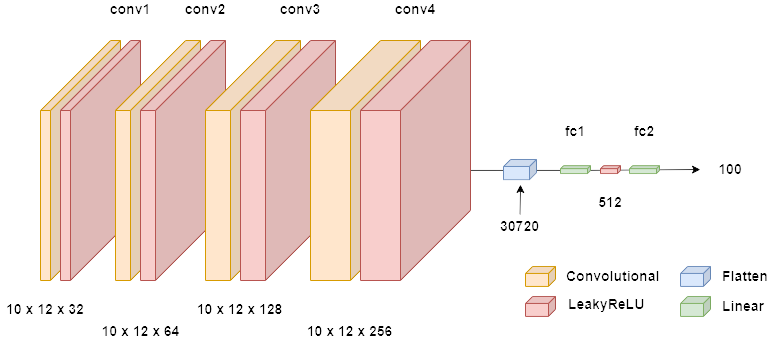
\includegraphics[width=0.9\linewidth]{images/convDQN.png}
            \caption{Convolution Policy Network Architecture.}
            \label{fig:convDQN}
        \end{figure}
        %
        
        \noindent
        The input tensor has dimensions $10 \times 12$, where $|B|=10$ represents the number of blocks in the state and $|CR^*|=12$ represents the number of possible colors a block can have. Each block is encoded using one-hot encoding, meaning that each color is represented as a binary vector of length 12. The output is then flattened and passed through two \emph{fully connected} (FC) layers, which process the data to produce the final output, as shown in Figure~\ref{fig:convDQN}.\tinydouble

        \noindent
        Policy models are trained individually in the underlying game using the deep Q-learning reinforcement learning algorithm specified in Algorithm~\ref{alg:dqn_algorithm}. We set $\gamma$ to 0.7. To optimize the model parameters, we use the smooth L1 loss function with $\beta$=1.0 and the Adam optimizer with a learning rate of 5e-4 and weight decay of 1e-5 to prevent over-fitting. To further enhance the learning process, we incorporate experience replay, with a memory that stores up to 10 million experiences \cite{10.1007/BF00992699}. A target network alongside the main policy network, is being used according to the \emph{Double-DQN} approach \cite{vanhasselt2015deep}. To update the target network we apply a soft update with a factor $\tau$=5e-3. This gradually brings the target network closer to the policy network, balancing learning speed and stability. With a batch size of 64, we train the models for 10,000 episodes.
        %
        \begin{algorithm}
            \caption{Double Deep Q-Learning with Experience Replay}
            \label{alg:dqn_algorithm}
            \begin{algorithmic}[1]
            \State $Q_\theta$, $Q_{\theta'} \gets Q_\theta$, $M$ \Comment{Initialize policy/target nets \& memory}
            \For{episode}
                \State $s \gets s_{0}$
                \For{step}
                    \State $a \gets \text{argmax}_a Q_\theta(s)$ \Comment{Select $\epsilon$-greedy action}
                    \State $(s, a, r, s') \in M$ \Comment{Store experience}
                    \If{$|M| > \text{batch size}$} 
                        \For{each $(s, a, r, s')$ in $M$} \Comment{Sample memory}
                            \State $y \gets r + \gamma \max_{a'} Q_{\theta'}(s')$
                            \State $L \gets \text{Loss}(Q_\theta(s), y)$
                            \State $\theta \gets \theta - \alpha \nabla_\theta L$
                        \EndFor
                    \EndIf
                    \State $Q_{\theta'} \gets \tau Q_\theta + (1 - \tau) Q_{\theta'}$ \Comment{Soft update}
                    \State $s \gets s'$
                \EndFor
            \EndFor
            \end{algorithmic}
        \end{algorithm}
        %

        \noindent
        In this setup, the agents are trained without any co-players, meaning that each model learns in isolation. This approach is intentional, as our goal is to develop agents that play optimally on their own, rather than in collaboration with others. The idea is to explore how different styles of independent players interact with each other. We expect that some styles will lead to more conflicts than others, and this behavior is key to our analysis. If we had trained the agents together, for example using a \emph{multi-agent reinforcement learning} (MARL) approach designed for collaborative settings, the resulting agents would have learned joint policies, which would defeat the very purpose of evaluating how their individual  policies affect collaboration.\tinydouble

        \noindent
        Let us consider, for instance, the simulation statistics of two relatively compatible play styles that we expect to perform well together in the game: Player W (a robot player with preferences for warm color tones) and player C (a human with preferences for cool color tones). In Figure~\ref{fig:cw-solution}, we observe how these players' individual preferences shape their interactions.
        %
        \begin{figure}[H]
            \centering
            
\includegraphics[width=0.5\textwidth]{images/cw-solution.png}
            \caption{Example solution to the game showing how C player and W player interact based on their preferences.}
            \label{fig:cw-solution}
        \end{figure}
        %
        
        \noindent
        The statistics in Figure~\ref{fig:cw-stats} reveal the most frequently selected actions in terms of blocks and colors. Player C prefers colors like blue, purple, and green, while player W tends to choose colors like brown, orange, and red. Given these preferences, conflicts are unlikely to arise from color selection alone. Even in scenarios where they may choose to color neighboring blocks, it is highly impossible that both players will choose the same color.
        %
        \begin{figure}[H]
            \centering
            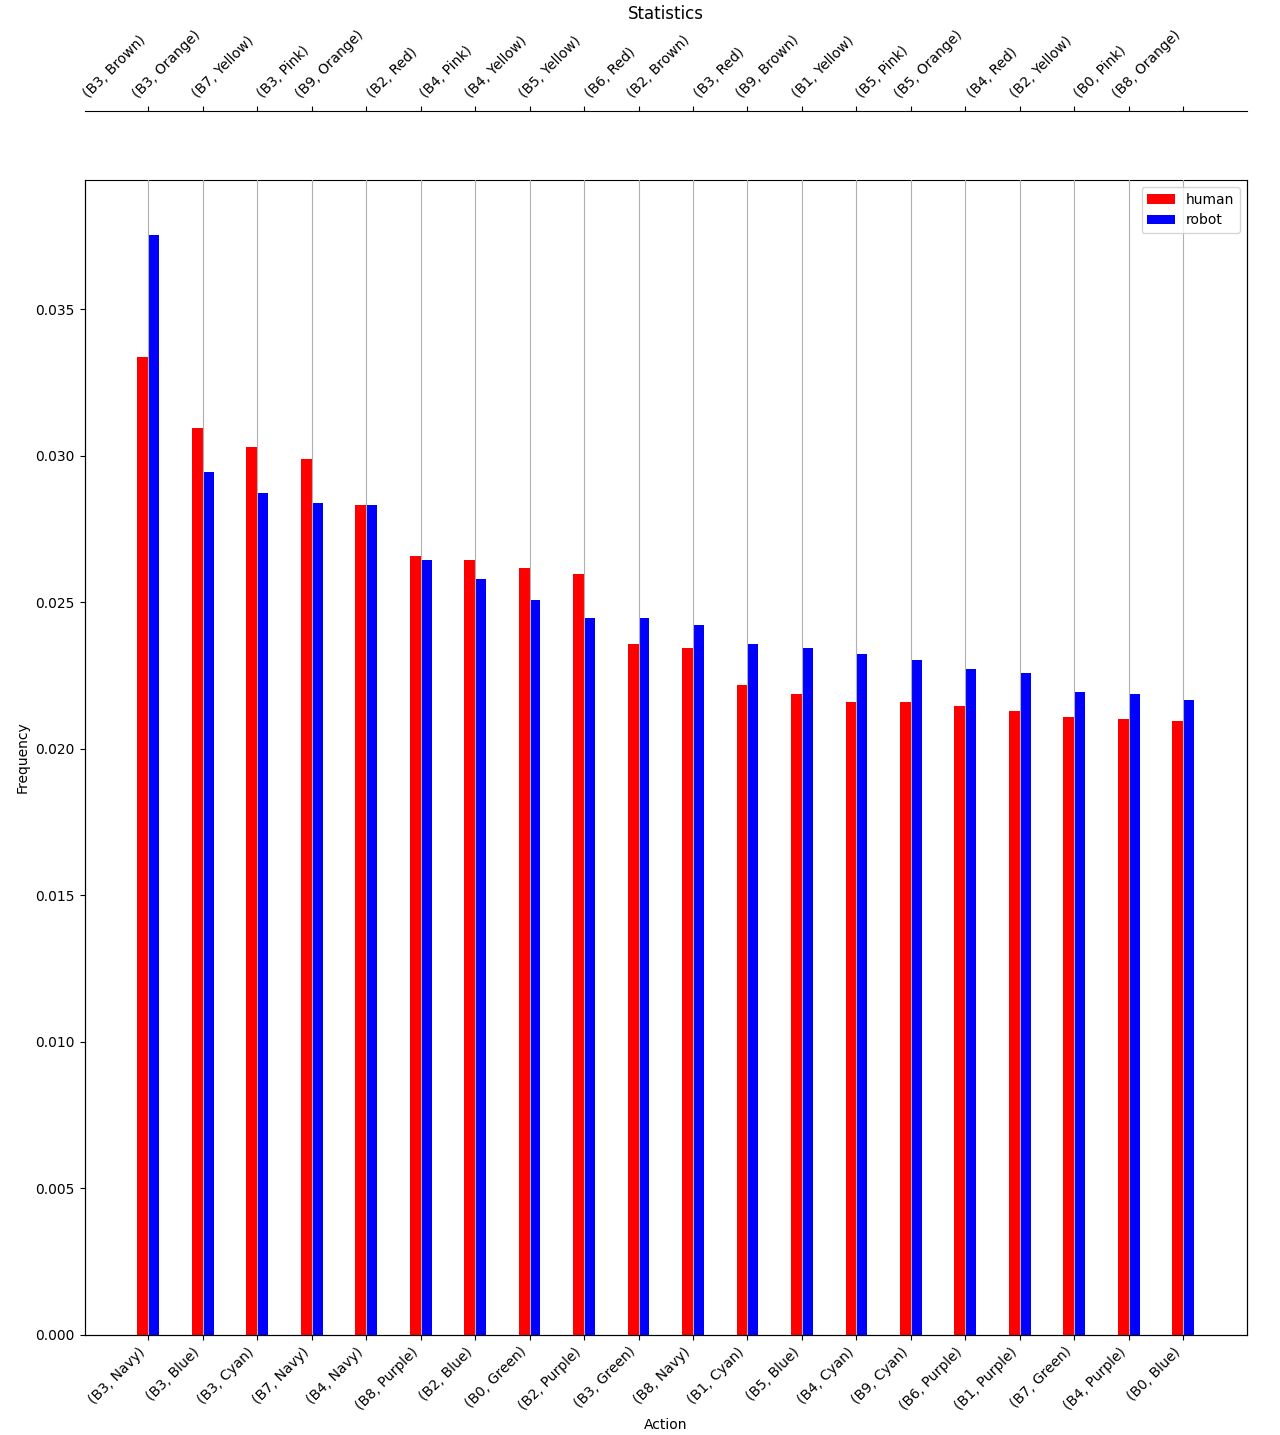
\includegraphics[width=0.9\textwidth]{images/cw-stats.png}
            \caption{Statistical analysis of the most frequently selected actions by C player and W player.}
            \label{fig:cw-stats}
        \end{figure}
        %        

        \noindent
        On the other hand, in Figure~\ref{fig:cc-solution}, we observe the interactions between two C players. In this case, we expect more conflicts, as both players share similar color preferences. This increases the likelihood of both players selecting the same color for neighboring blocks.
        %
        \begin{figure}[H]
            \centering
            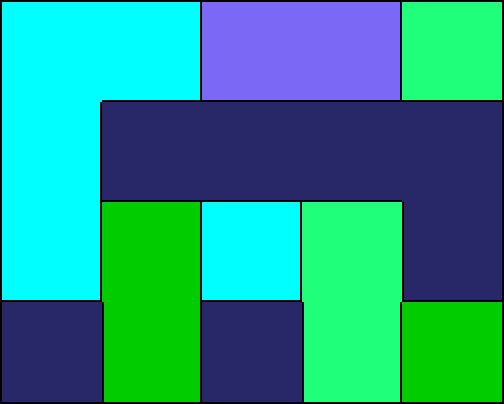
\includegraphics[width=0.5\textwidth]{images/cc-solution.png}
            \caption{Example solution to the game showing how two C players interact based on their preferences.}
            \label{fig:cc-solution}
        \end{figure}
        %
        
        \noindent
        The statistics shown in in Figure~\ref{fig:cc-stats} further support this, as they reveal a high probability of color overlap, primarily due to the dominance of cool colors in both action spaces. However, these conflicts are not a result of insufficient training, but rather stem from the inherent similarity in preferences.
        %
        \begin{figure}[H]
            \centering
            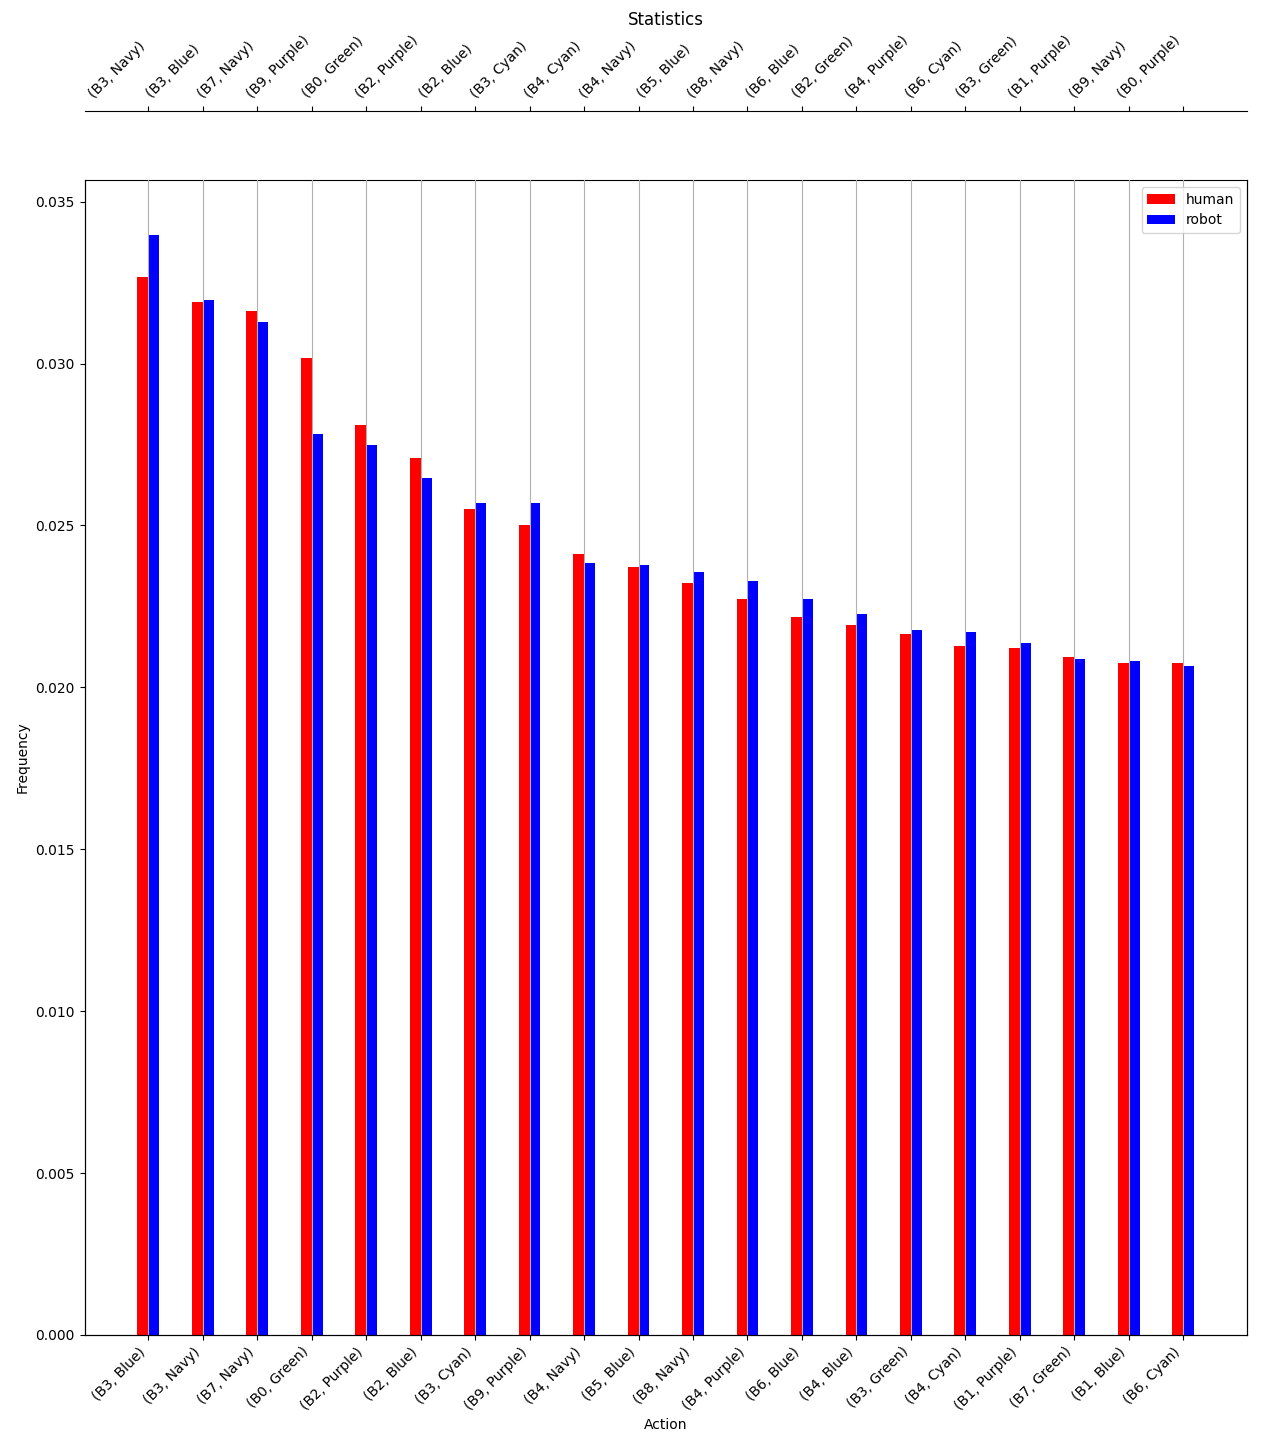
\includegraphics[width=0.9\textwidth]{images/cc-stats.png}
            \caption{Statistical analysis of the most frequently selected actions by two C players.}
            \label{fig:cc-stats}
        \end{figure}
        %   

        \noindent
        Other than that, both agents have been thoroughly trained in isolation, exploring a wide range of states and ultimately converging to stable policies. This allows them to respond effectively and optimally, even when paired with agents with conflicting styles of play. Therefore, even in the case of the most incompatible pairings, the number of mistakes remains minimal, and these mistakes are not due to inadequate exploration, but rather to the inherent conflicts in the agents’ preferences. 

    \subsubsection{Extracting the Empirical Payoff Matrix}

        We generate the empirical payoff matrix by simulating each strategy profile over multiple games. These payoffs represent how well different styles of play perform jointly, according to the game’s rules.\tinydouble

        \noindent
        The values in the payoff matrix are computed in terms of the delay and the quality of the solution according to the game's constraints (gain, penalty, and sanction), excluding preferences. This ensures a common ground for distinct strategies, evaluating solutions solely based on the game's rules. For each pair of strategies, we simulate the game over 5,000 repeats and calculate the average payoff for each strategy. These values are then organized into the payoff matrix, which is provided in Table~\ref{tab:gcg_payoff_matrix}. Each entry in the matrix represents the payoffs of strategies in the corresponding profile, with the first value indicating the payoff of the row player and the second value of the column player. The Nash equilibria are highlighted in bold, while nine of the top-ranked strategy profiles in the MCC are shaded in gray.
        %
        \begin{table}[h!]
            \centering
            \caption{Empirical Payoff Matrix for the Graph Coloring Game.}
            \label{tab:gcg_payoff_matrix}
            \vspace{0.5em}
            \resizebox{\textwidth}{!}{%
            \begin{tabular}{lccccccccccc}
                \hline
                    & A & AE & C & CA & E & I & L & LE & M & W & WL \\
                \hline
                A  & (3.12, 3.11) & (3.15, 3.16) & (3.17, 3.17) & (3.14, 3.17) & (3.16, 3.17) & (3.16, 3.15) & (3.22, 3.13) & (3.19, 3.16) & (3.15, 3.18) & (3.16, 3.17) & (3.21, 3.18) \\
                
                AE & (3.17, 3.17) & (3.11, 3.11) & (3.18, 3.17) & \cellcolor{gray!16}(3.15, 3.17) & (3.17, 3.16) & (3.19, 3.16) & (3.23, 3.12) & (3.19, 3.16) & \cellcolor{gray!16}(3.15, 3.18) & (3.17, 3.17) & (3.20, 3.16) \\
                
                C  & (3.17, 3.16) & (3.16, 3.17) & (3.10, 3.10) & (3.14, 3.17) & (3.15, 3.15) & (3.18, 3.15) & (3.22, 3.12) & (3.17, 3.14) & (3.14, 3.17) & (3.17, 3.16) & (3.20, 3.17) \\
                
                CA & (3.17, 3.15) & (3.17, 3.15) & (3.17, 3.14) & (3.11, 3.11) & (3.18, 3.15) & (3.18, 3.14) & (3.24, 3.13) & \cellcolor{gray!16}(3.21, 3.16) & \cellcolor{gray!16}(3.16, 3.16) & (3.19, 3.16) & \cellcolor{gray!16}(3.22, 3.15) \\
                
                E  & (3.15, 3.16) & (3.16, 3.16) & (3.15, 3.16) & \cellcolor{gray!16}(3.15, 3.17) & (3.10, 3.10) & (3.18, 3.16) & (3.22, 3.12) & (3.19, 3.14) & (3.15, 3.17) & (3.16, 3.17) & (3.19, 3.17) \\
                
                I  & (3.14, 3.16) & (3.16, 3.18) & (3.16, 3.18) & (3.15, 3.19) & (3.16, 3.17) & (3.12, 3.12) & (3.22, 3.14) & (3.18, 3.16) & (3.14, 3.19) & (3.16, 3.18) & (3.19, 3.18) \\

                L  & (3.14, 3.22) & (3.11, 3.22) & (3.12, 3.22) & (3.13, 3.23) & (3.12, 3.22) & (3.13, 3.22) & (3.12, 3.12) & (3.14, 3.20) & (3.11, 3.21) & (3.14, 3.23) & \textbf{(3.15, 3.21)} \\
                
                LE & (3.15, 3.19) & (3.14, 3.18) & (3.14, 3.18) & (3.15, 3.21) & (3.15, 3.19) & (3.16, 3.17) & (3.20, 3.14) & (3.11, 3.11) & (3.14, 3.22) & (3.15, 3.18) & (3.18, 3.19) \\
                
                M  & (3.17, 3.14) & (3.17, 3.15) & (3.17, 3.15) & \cellcolor{gray!16}(3.16, 3.17) & (3.16, 3.14) & (3.18, 3.14) & (3.23, 3.11) & (3.20, 3.14) & (3.06, 3.08) & (3.18, 3.15) & (3.20, 3.16) \\
                
                W  & (3.17, 3.17) & (3.17, 3.18) & (3.16, 3.18) & \cellcolor{gray!16}(3.16, 3.20) & (3.17, 3.17) & (3.18, 3.16) & (3.21, 3.13) & (3.18, 3.15) & (3.15, 3.18) & (3.08, 3.09) & (3.19, 3.15) \\
            
                WL & (3.17, 3.20) & (3.17, 3.19) & (3.17, 3.19) & (3.17, 3.22) & (3.17, 3.19) & (3.18, 3.19) & \textbf{(3.21, 3.15)} & (3.19, 3.17) & \cellcolor{gray!16}(3.16, 3.20) & (3.16, 3.19) & (3.13, 3.13) \\
                \hline
            \end{tabular}
            }
        \end{table}
        %

        \noindent
        From this matrix, we observe that (L, WL) and its symmetric counterpart (WL, L) both with payoffs of (3.15, 3.21) and (3.21, 3.15) respectively, are the only Nash equilibria. It is important to note here that these equilibria prescribe agents' strategies given that they do play the game with rational co-players, but they do not capture the overall dynamics of the game, considering the long-term effects of agents' interactions.

    \subsubsection{Evaluating and Ranking Joint Policies}

        Given the payoff matrix derived from the empirical analysis, we apply the \emph{$\alpha$-Rank} method to evaluate the performance of strategy profiles over time in terms of the MCC solution concept. Specifically, we ran the method 1,000 times, using values of $\alpha$ within the range $[0.1, 10]$ with step=0.01, while assuming populations of size $m=100$. We provide as input the strategies defined in Section~\ref{sec:5.1} and the empirical game payoff matrix. We focus on the rankings of the top 6 strategy profiles, to identify the stronger ones across different values of $\alpha$.\tinydouble

        \noindent
        As we observe from the rankings in Table~\ref{tab:ranking_table}, the strategy profile that prevails in the long run is (WL, CA); this is the primary component of the MCC. Although the table was derived using an $\alpha$ value of 2, the rankings remain consistent even when $\alpha$ is set to 10. We choose $\alpha=2$ over $\alpha=10$, to display the rankings of lower-performing strategy profiles, which would otherwise drop to zero. First, it is worth mentioning that the Nash equilibria (L, WL) and (WL, L) don't appear among the top-ranked strategy profiles. This is because MCC components are defined based on how well strategies perform when interacting with other strategies, based on long-term agents interactions. The individual strategies within the Nash equilibrium profile, either WL or L, may not result in favorable interactions with other strategies. As a result, the profile (WL, L) is ranked lower that others.
        %
        \begin{table}[H]
            \centering
            \caption{Rankings for $\alpha=2$.}
            \label{tab:ranking_table}
            \vspace{0.5em}
            \begin{tabular}{lcc}
                \hline
                \textbf{Agent} & \textbf{Rank} & \textbf{Score} \\
                \hline
                (WL, CA) & 1 & 0.42 \\
                (W, CA) & 2 & 0.13 \\
                (M, CA) & 3 & 0.12 \\
                (CA, M) & 4 & 0.08 \\
                (CA, W) & 5 & 0.08 \\
                (CA, LE) & 6 & 0.01 \\
                \hline
            \end{tabular}
        \end{table}
        %

        \noindent
        To further support our observations regarding the misalignment between the two solution concepts, let's examine why (CA, WL) is part of the MCCs, while (L, WL), the Nash equilibrium, is not. A closer look at the payoff matrix in Table~\ref{tab:gcg_payoff_matrix} reveals that L appears to be the worst-performing strategy for the row player, with an average payoff of 3.13. In this case, being in the Nash equilibrium means the player is stuck with a strategy that gives low rewards, making it the best among other options, rather than a strong choice. If it happens to play this strategy, it would expect its rational opponent to play WL. Strategy CA on the other hand, is the best-performing strategy for the row player, with an average payoff of 3.18. Combined with WL, which is the best performing strategy for the column player, with an average payoff of 3.18, they make profile (CA, WL) becomes the top ranked strategy profile in the ranking Table~\ref{tab:ranking_table}.\tinydouble

        \noindent
        Rankings within the MCC are also very intuitive. For example, strategies that prefer different color tones, such as (WL, CA) or (W, CA), tend to result into fewer conflicts since, they naturally avoid selecting the same colors. Similarly, strategies that prefer different blocks based on their difficulty, such as (WL, CA) or (CA, LE), tend to provide solutions with minimal delay, as they naturally avoid coloring the same blocks. Notably, profiles with mixed preferences across these dimensions demonstrate the most promising performance, which explains why (WL, CA), as such a profile, is a key component of the MCC. However, not all profile rankings can be easily explained through the game's rules alone; the expected influence of certain strategies on the quality of the solutions remains ambiguous. For example, profiles with strategies like M and E are more difficult to analyze.
        %
        \begin{figure}[H]
            \centering
            \begin{subfigure}[b]{0.45\linewidth}
                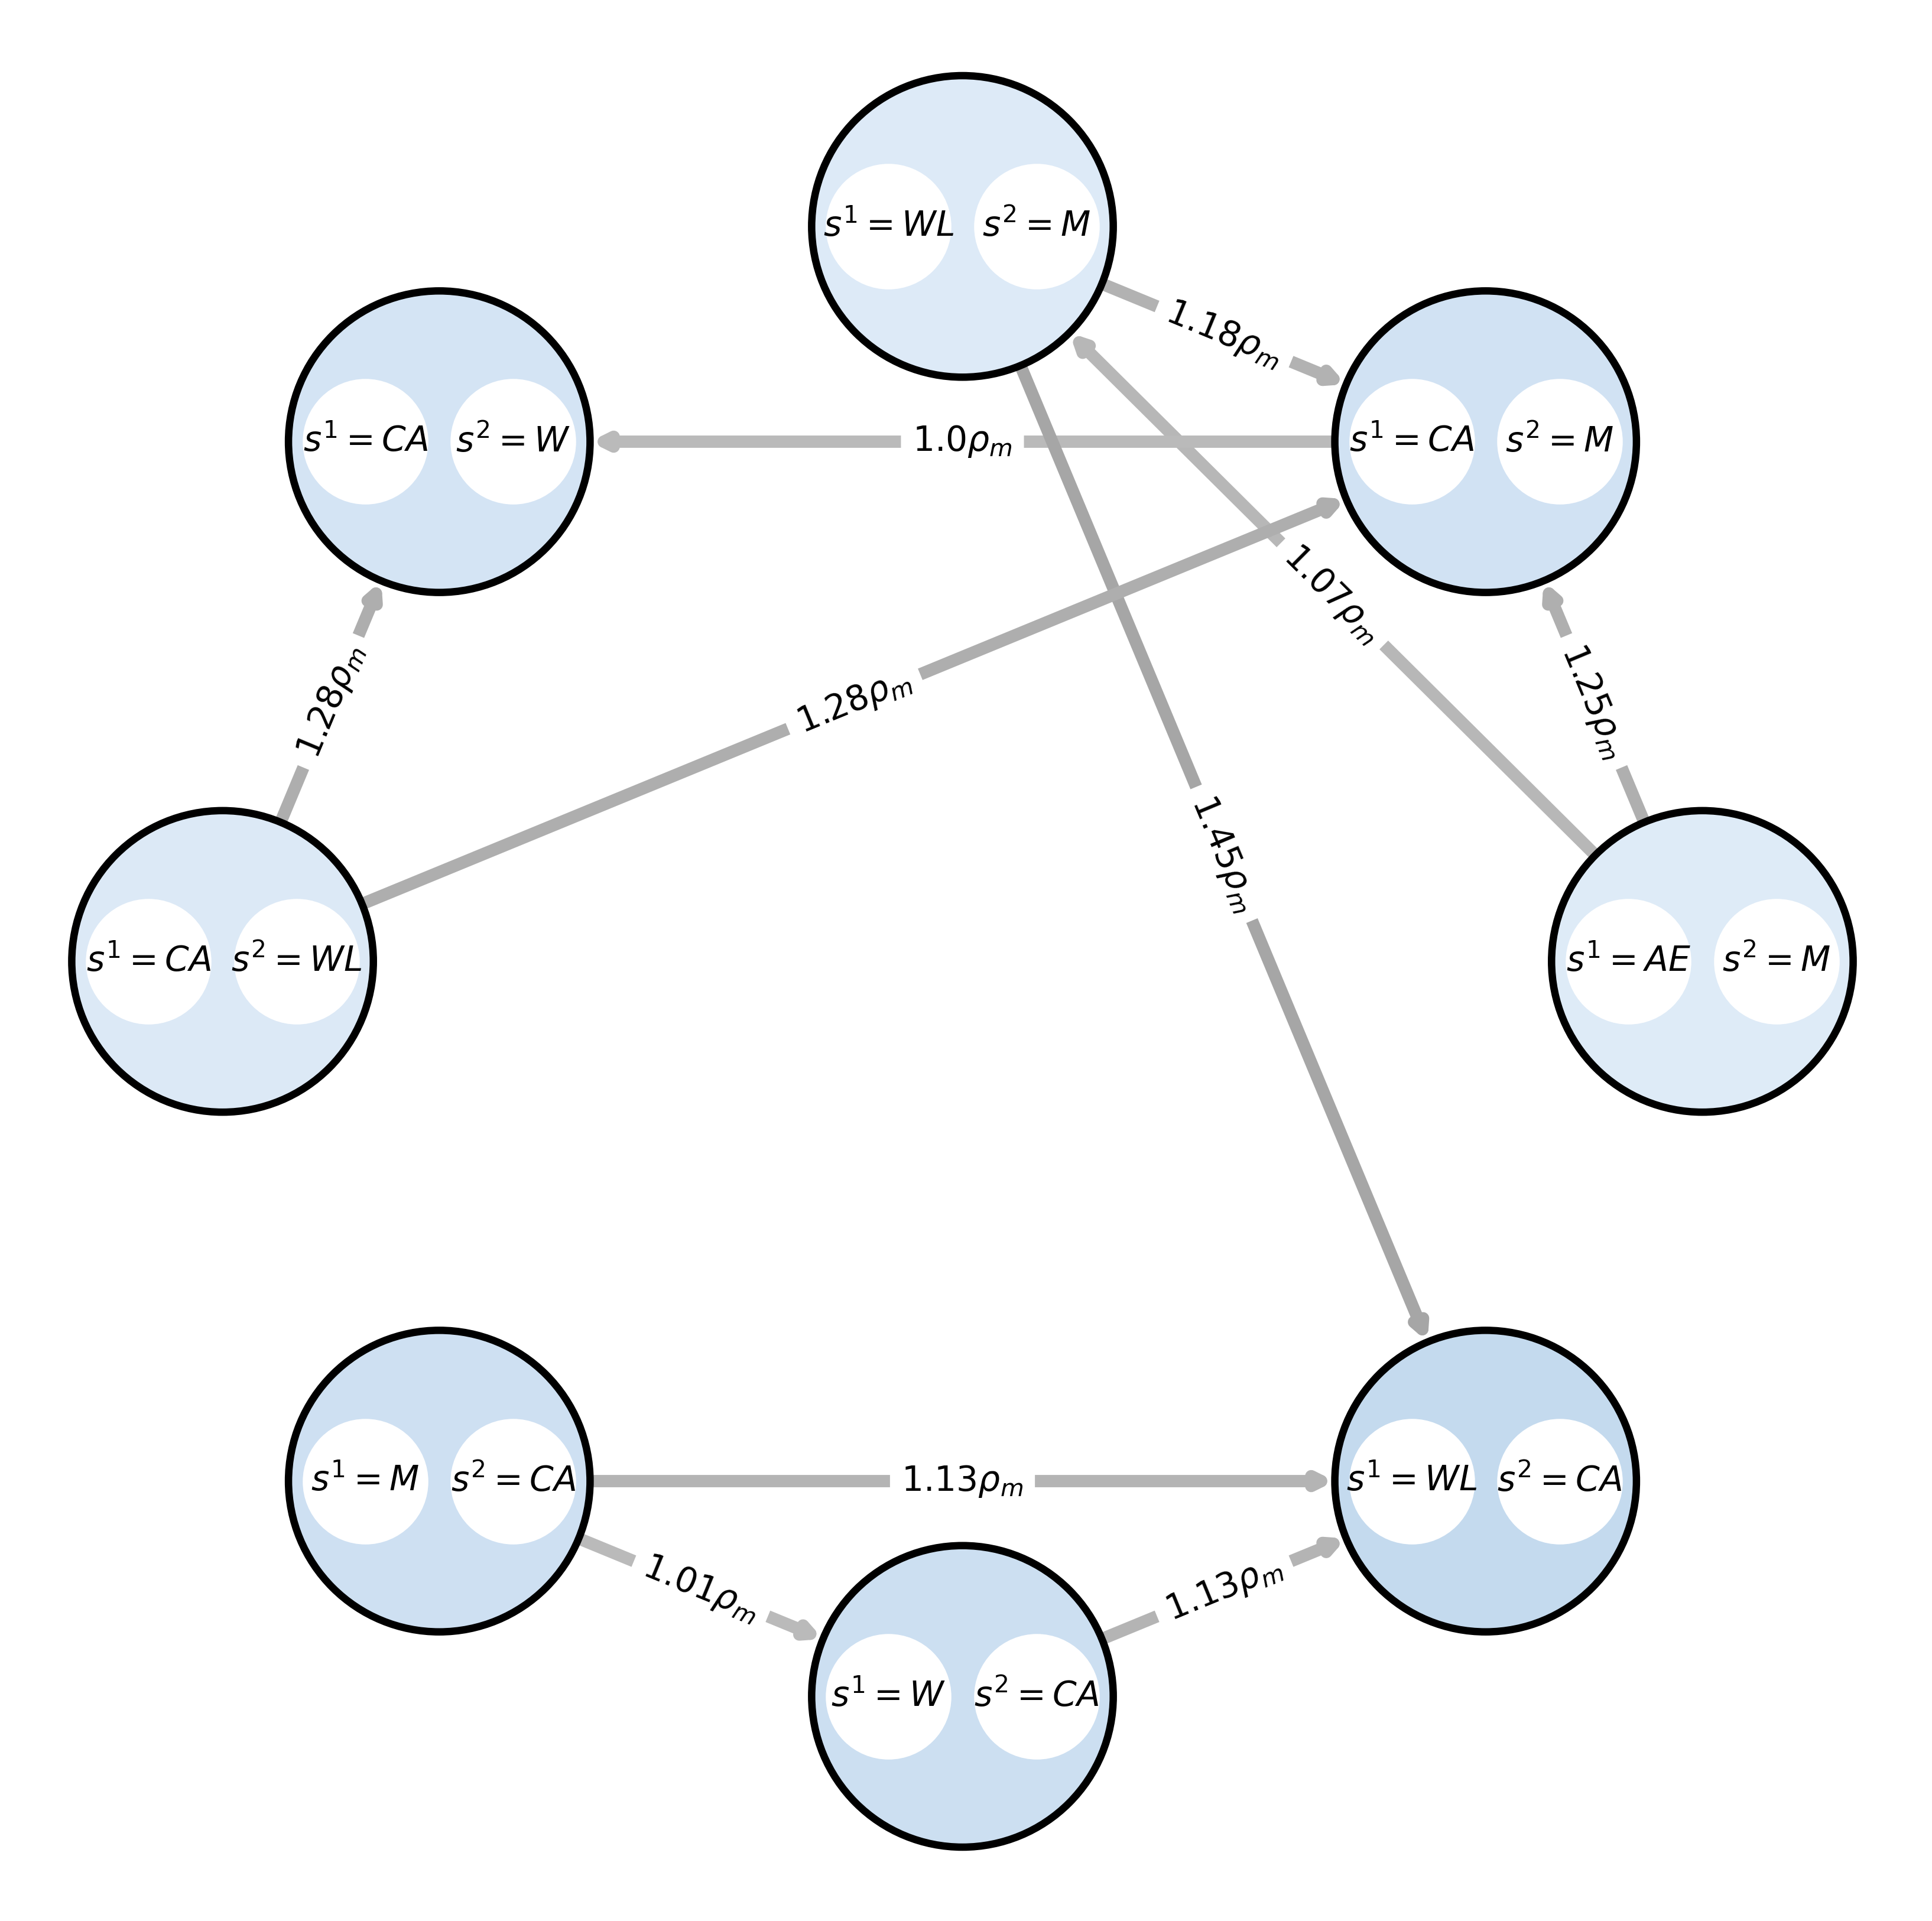
\includegraphics[width=\linewidth]{images/rg_0.4.png}
                \caption{$alpha=0.4$}
                \label{fig:response_graph_0.4}
            \end{subfigure}
            \hfill
            \begin{subfigure}[b]{0.45\linewidth}
                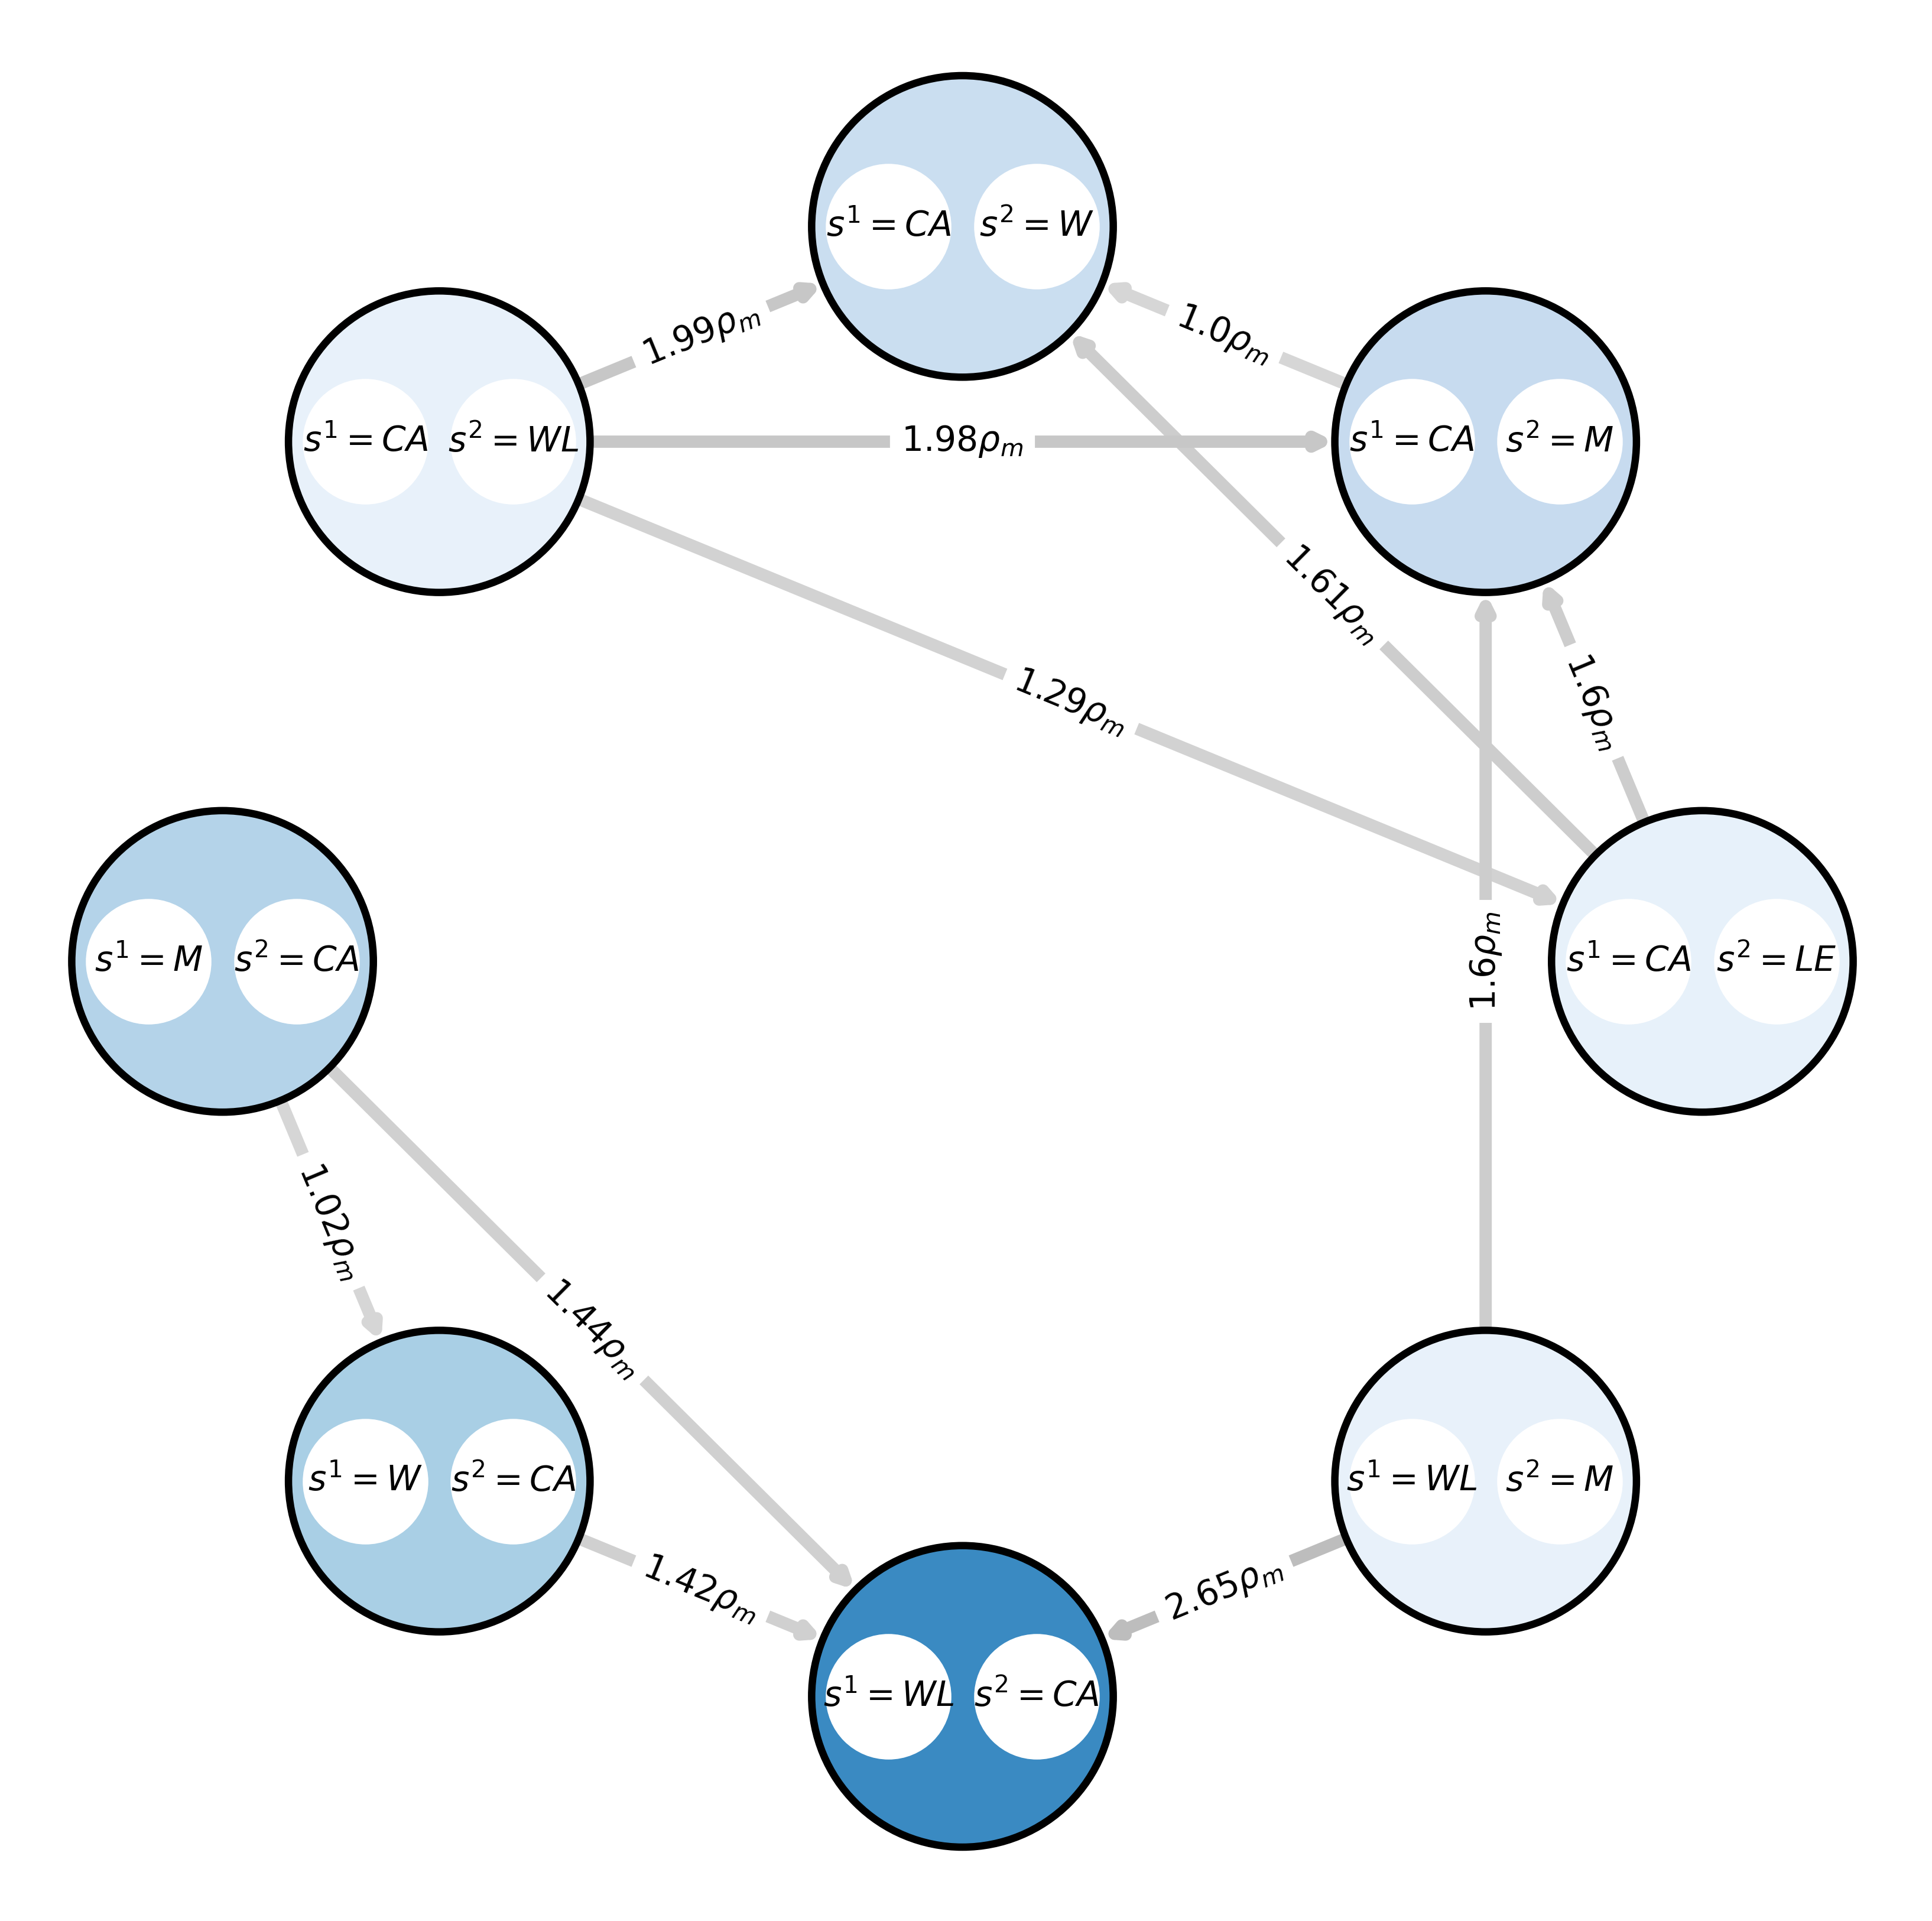
\includegraphics[width=\linewidth]{images/rg_1.3.png}
                \caption{$alpha=1.3$}
                \label{fig:response_graph_1.3}
            \end{subfigure}

            \begin{subfigure}[b]{0.45\linewidth}
                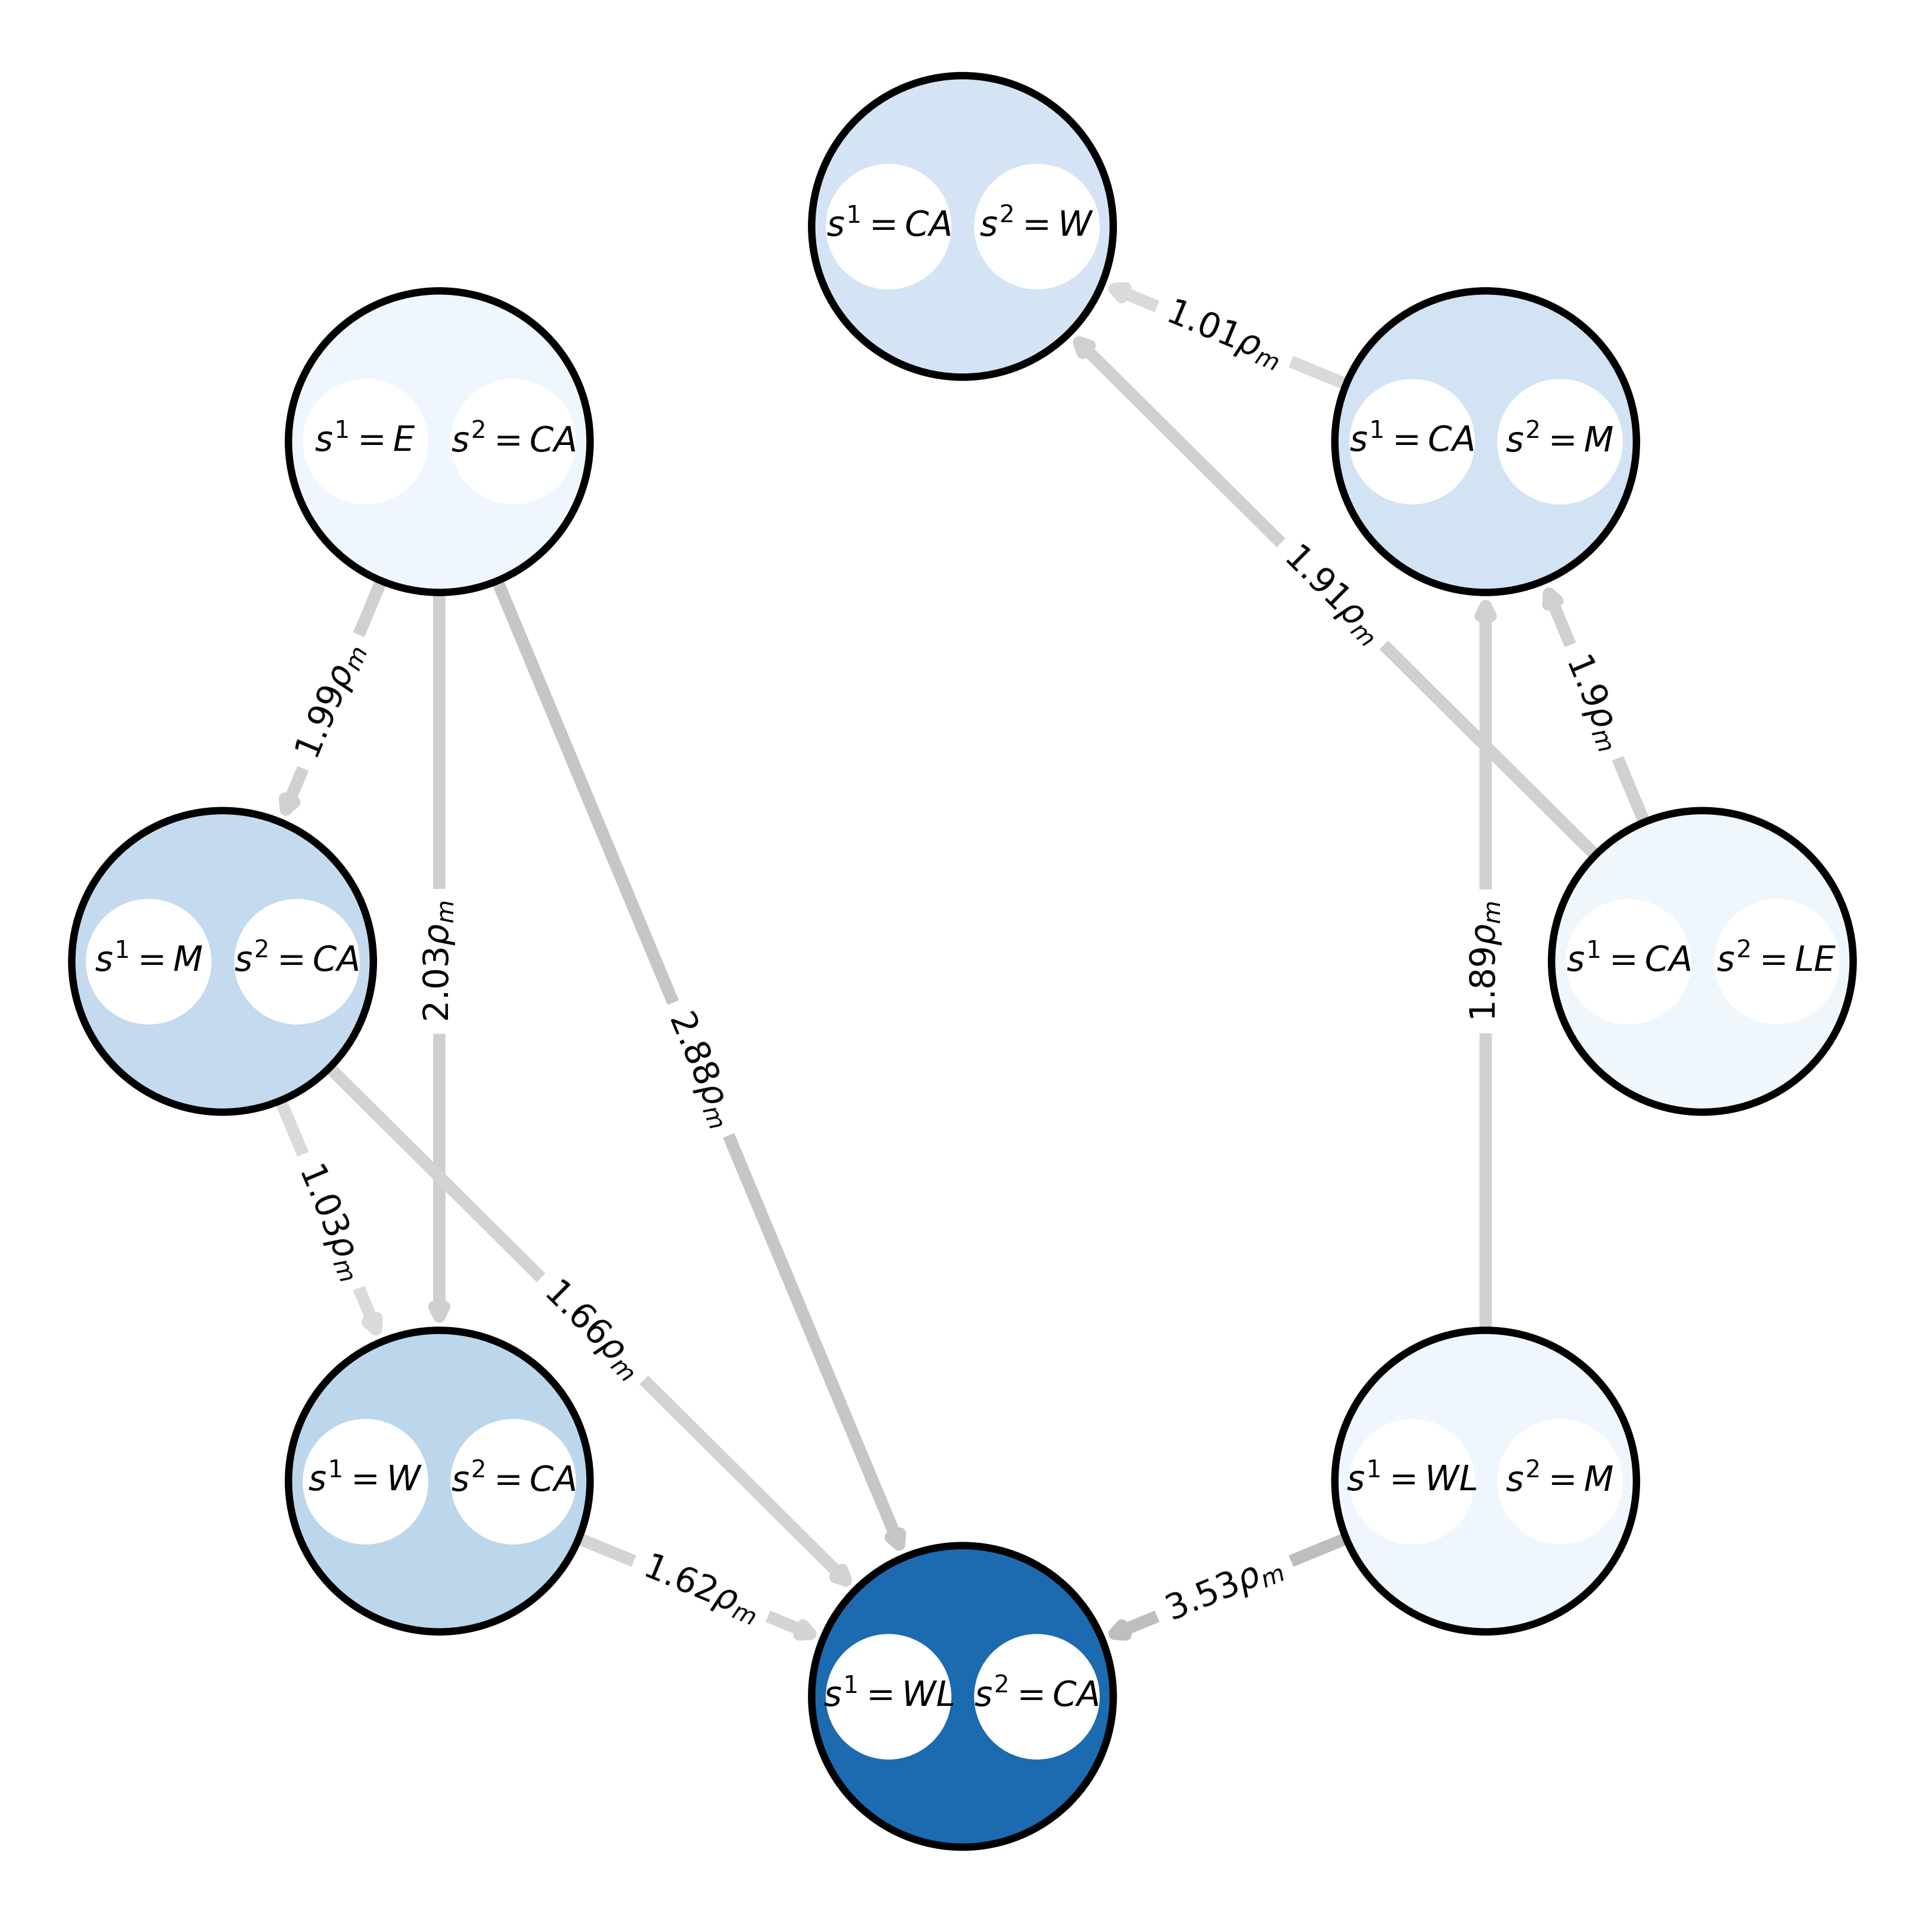
\includegraphics[width=\linewidth]{images/rg_1.9.png}
                \caption{$alpha=1.9$}
                \label{fig:response_graph_1.9}
            \end{subfigure}
            \hfill
            \begin{subfigure}[b]{0.45\linewidth}
                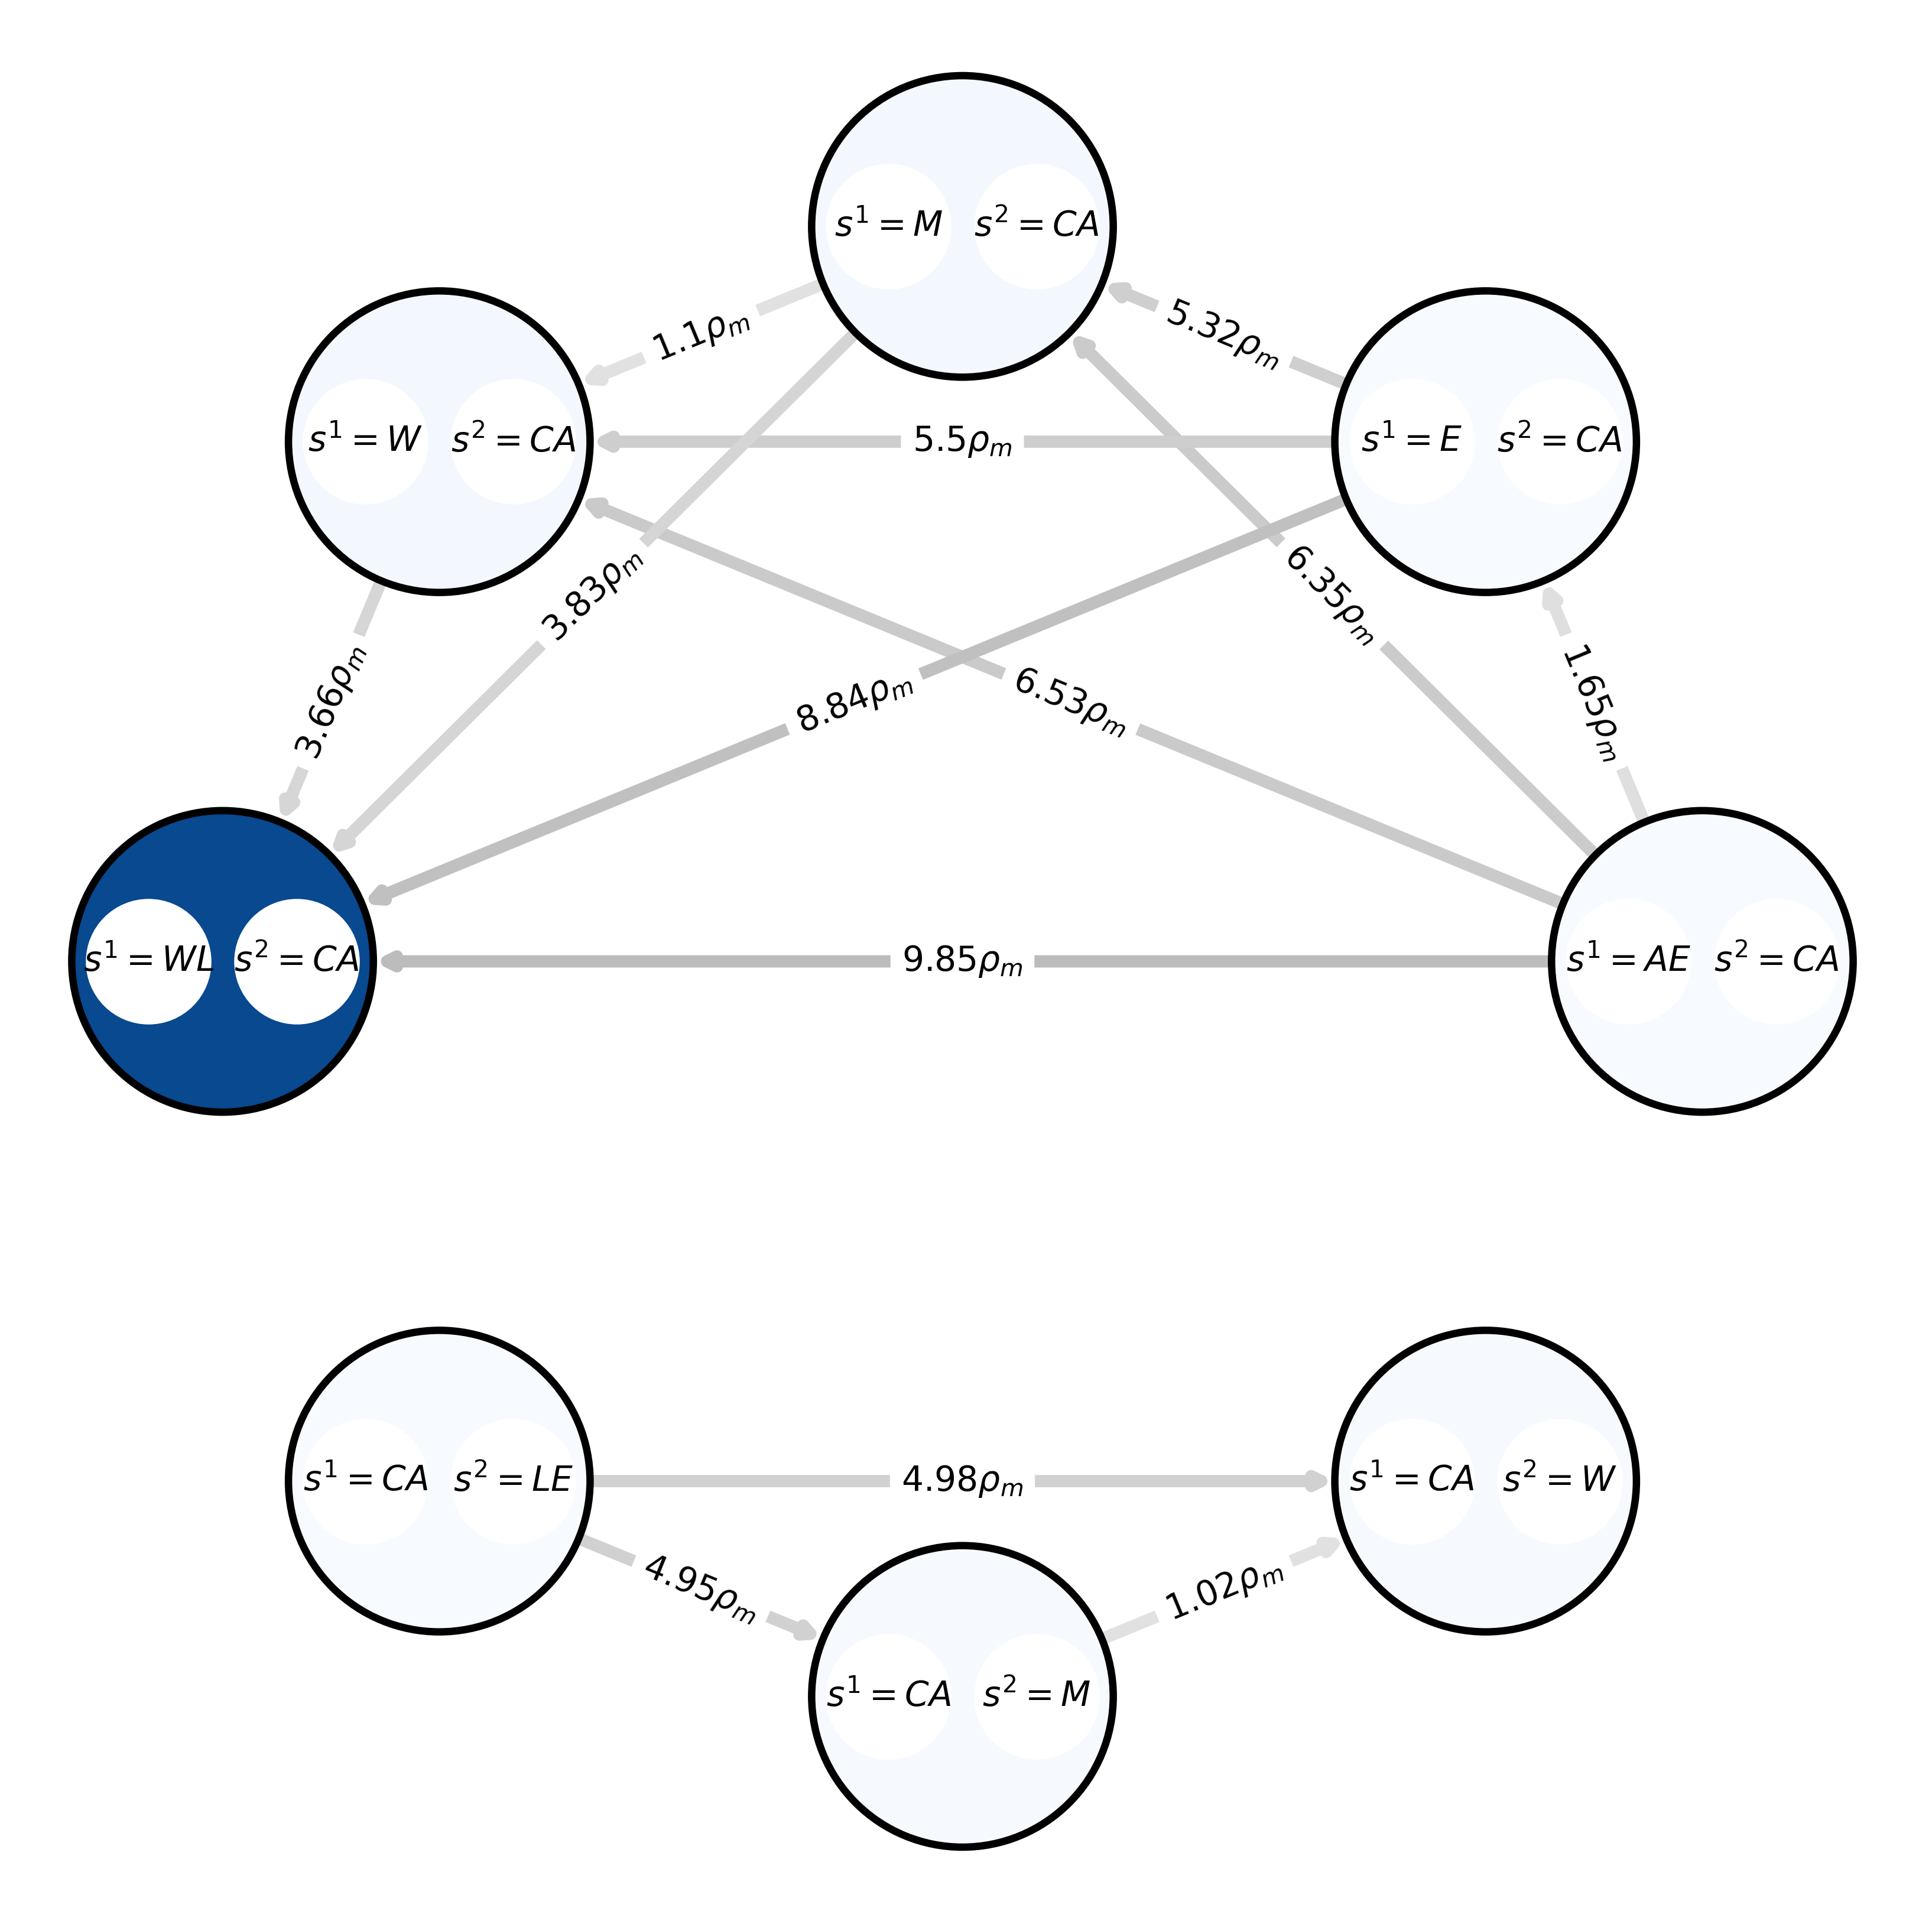
\includegraphics[width=\linewidth]{images/rg_6.4.png}
                \caption{$alpha=6.4$}
                \label{fig:response_graph_6.4}
            \end{subfigure}

            \caption{Response graphs of strategy profiles' dynamics.}
            \label{fig:response_graphs}
        \end{figure}
        %

        \noindent
        The response graph provides a visualization to interpret the \emph{$\alpha$-Rank} results. This graph illustrates the MCC, using the strategy profiles' masses from the stationary distribution, $\pi$, along with the fixation probability function $\rho$ provided by \emph{$\alpha$-Rank}. Figure~\ref{fig:response_graphs} shows the response graphs for $\alpha = 0.4$, $1.3$, $1.9$ and $6.4$. We consider it to be part of the descriptive framework $\mathcal{D}$, as it offers insights into how rankings were derived.\tinydouble

        \noindent
        Each node in the graph represents a unique strategy profile in the MCC, while the edges indicate transitions between them. The values on the edges show the fixation probabilities normalized by the neutral fixation probability, denoted as $\rho_m$. The nodes and edges are color-coded. Darker blue nodes represent more strong joint profiles, while lighter blue nodes represent transient ones. Similarly, bold arrows suggest a strong advantage in shifting between the nodes, whereas faint ones suggest less of an advantage.\tinydouble

        \noindent
        The response graph describes the overall dynamics of the strategy profiles in the empirical game. One prominent feature is the primary component of the MCC, specifically the profile (WL, CA). This profile, indicated by a dark blue color, has multiple graph edges leading to it, while none from it, indicating that strategies in this profile are non-transient. This is further supported by the large fixation probabilities along the edges. A particularly prominent example is the cluster (CA, LE)-(CA, M)-(CA, W), which consists of three strongly connected profiles, indicating that once a player adopts one of these profiles, they will likely remain within their cluster. These components reflect stable regions in the game’s strategy dynamics, where transitions between profiles become locked into a cycle.\tinydouble

        \noindent
        To further investigate the effect of $\alpha$ on profile dominance, we plotted the stationary distribution $\pi$ across all $\alpha$ values used in the experiments, for the top-performing strategy profiles (see Figure~\ref{fig:alpha_x_pi}). This visualization —also part of $\mathcal{D}$— helps us understand how the stationary distribution changes as the selection intensity increases. The x-axis represents the different $\alpha$ values, ranging from $0.1$ to $3$ in Figure~\ref{fig:alpha_x_pi_3}, and from $0.1$ to $10$ in Figure~\ref{fig:alpha_x_pi_10}, while the y-axis in both figures shows the mass of each strategy profile in the stationary distribution $\pi$. As $\alpha$ increases, the distribution converges, indicating that the selection process stabilizes. The final mass distributions are highlighted in boxed regions. The legend on the right side of the plot displays the top-performing joint strategies, with the stronger ones appearing at the top.
        %
        \begin{figure}[H]
            \centering
            \begin{subfigure}[b]{0.49\linewidth}
                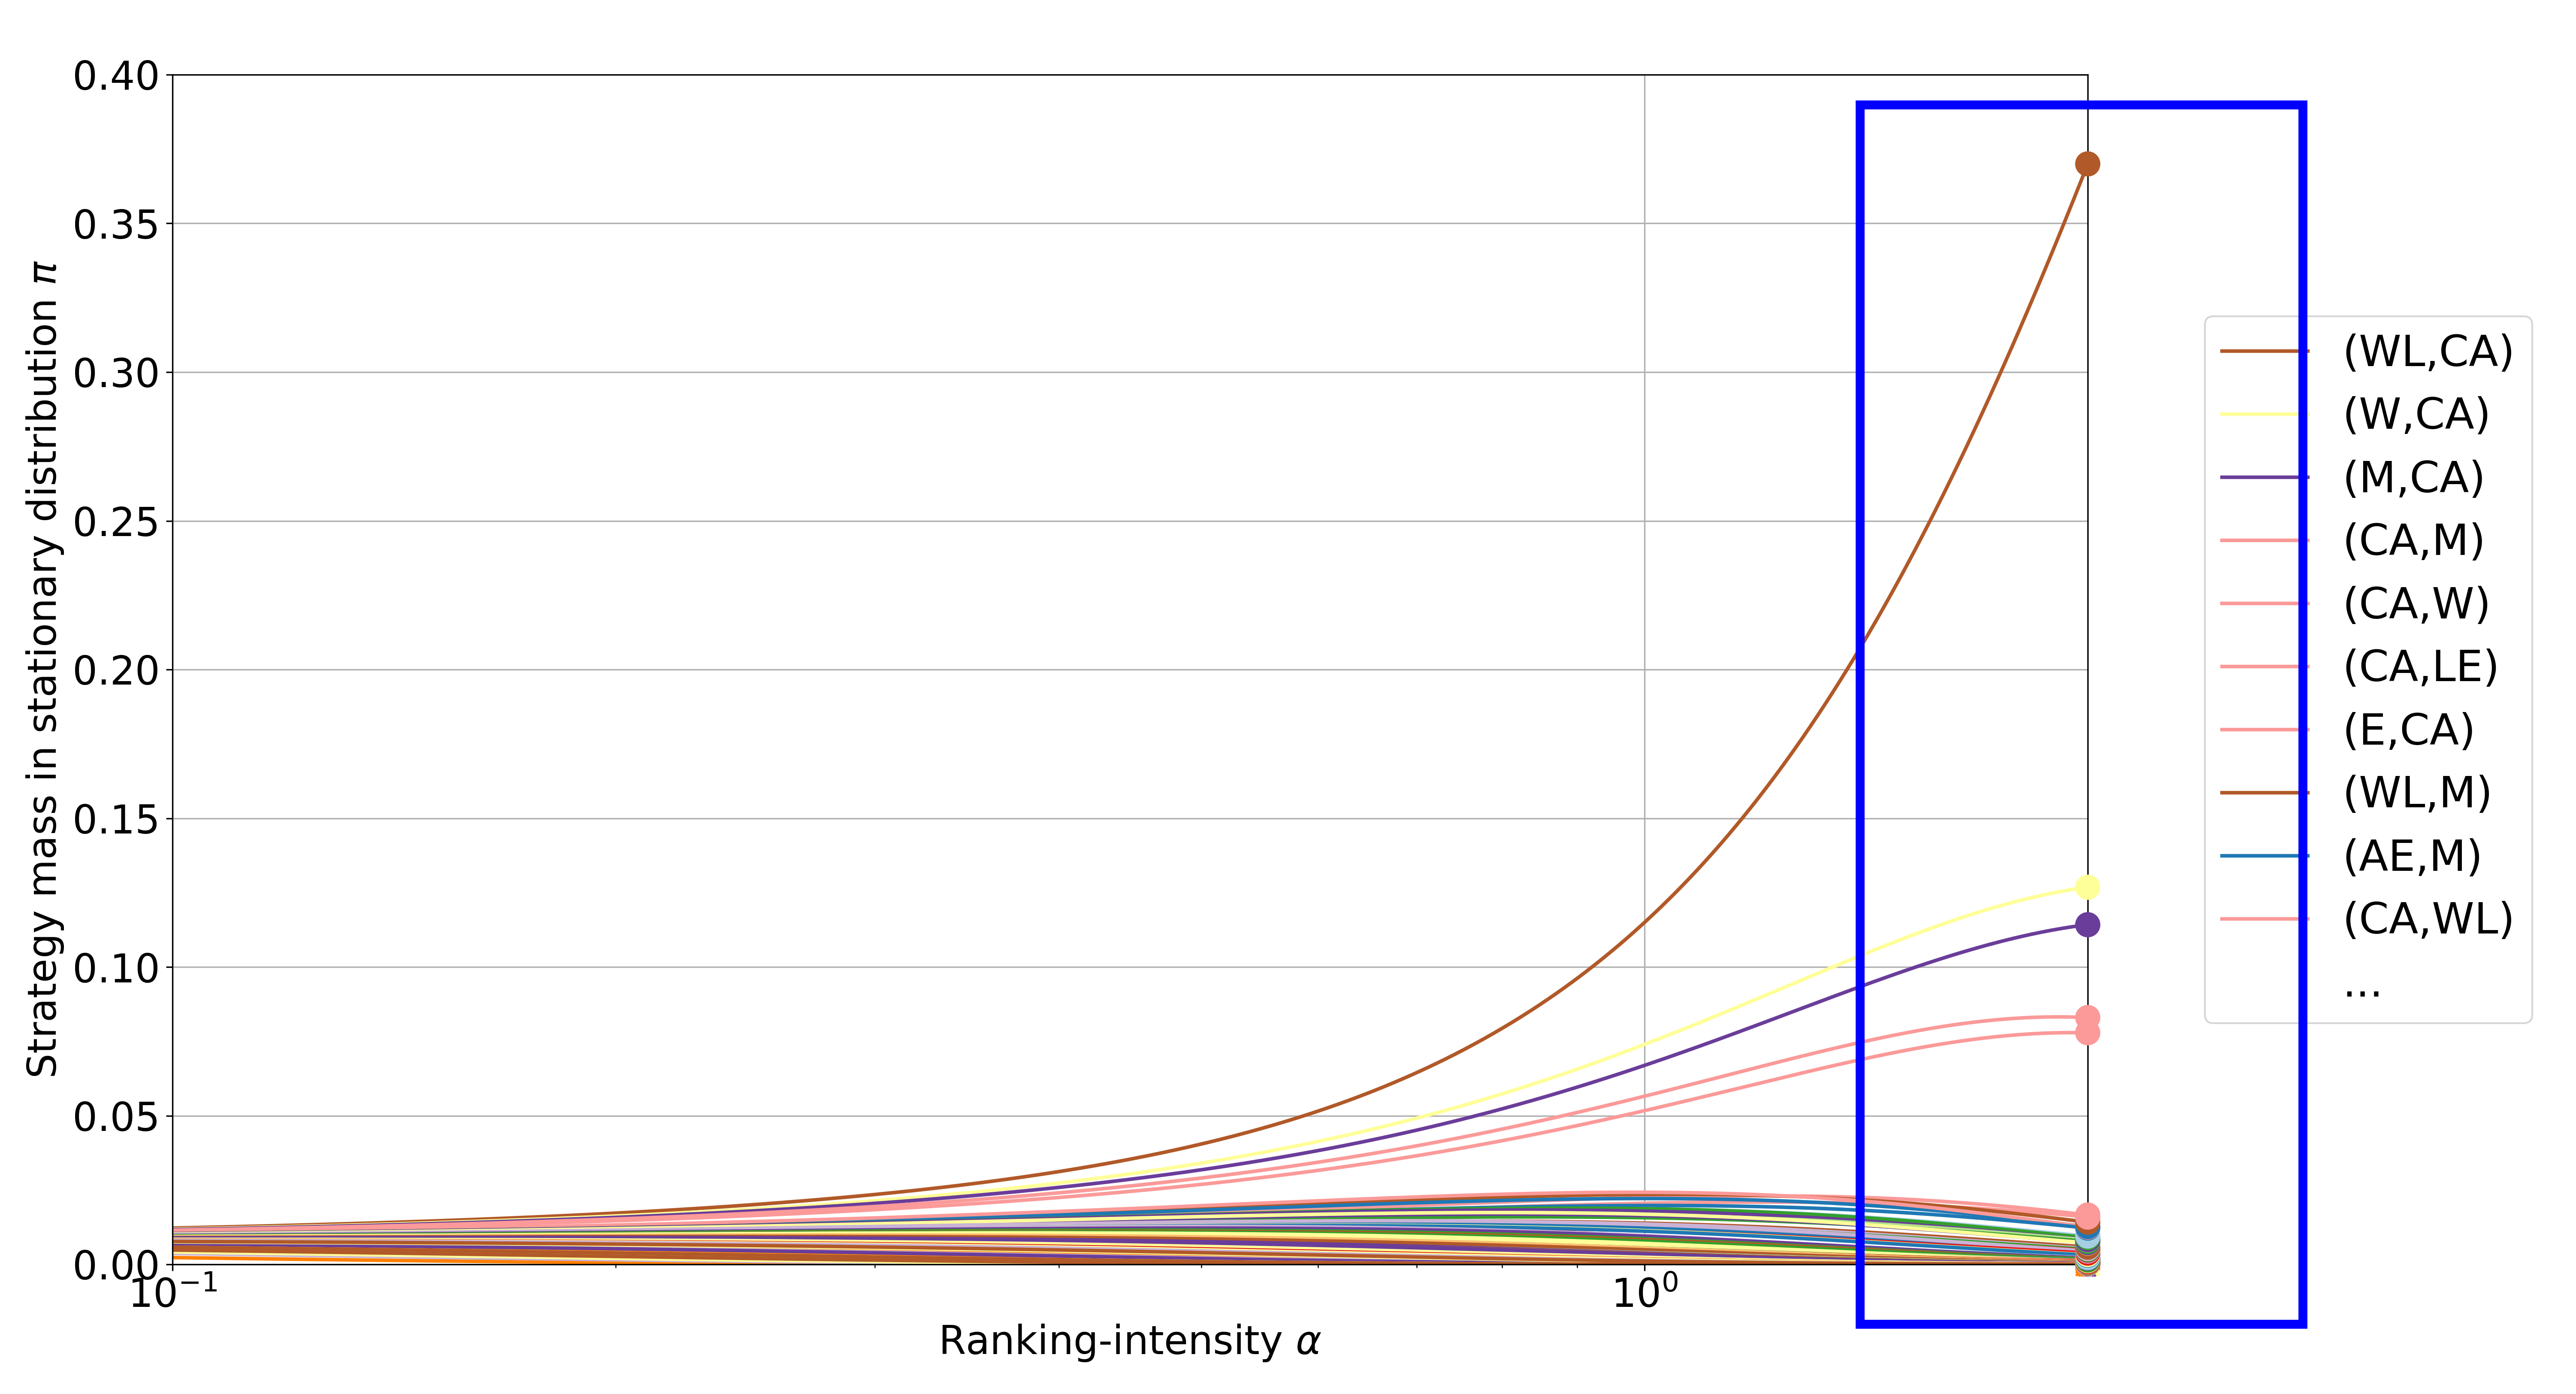
\includegraphics[width=\linewidth]{images/alpha_x_pi_3.png}
                \caption{Mass across $\alpha \in [0.1, 3]$.}
                \label{fig:alpha_x_pi_3}
            \end{subfigure}
            \hfill
            \begin{subfigure}[b]{0.49\linewidth}
                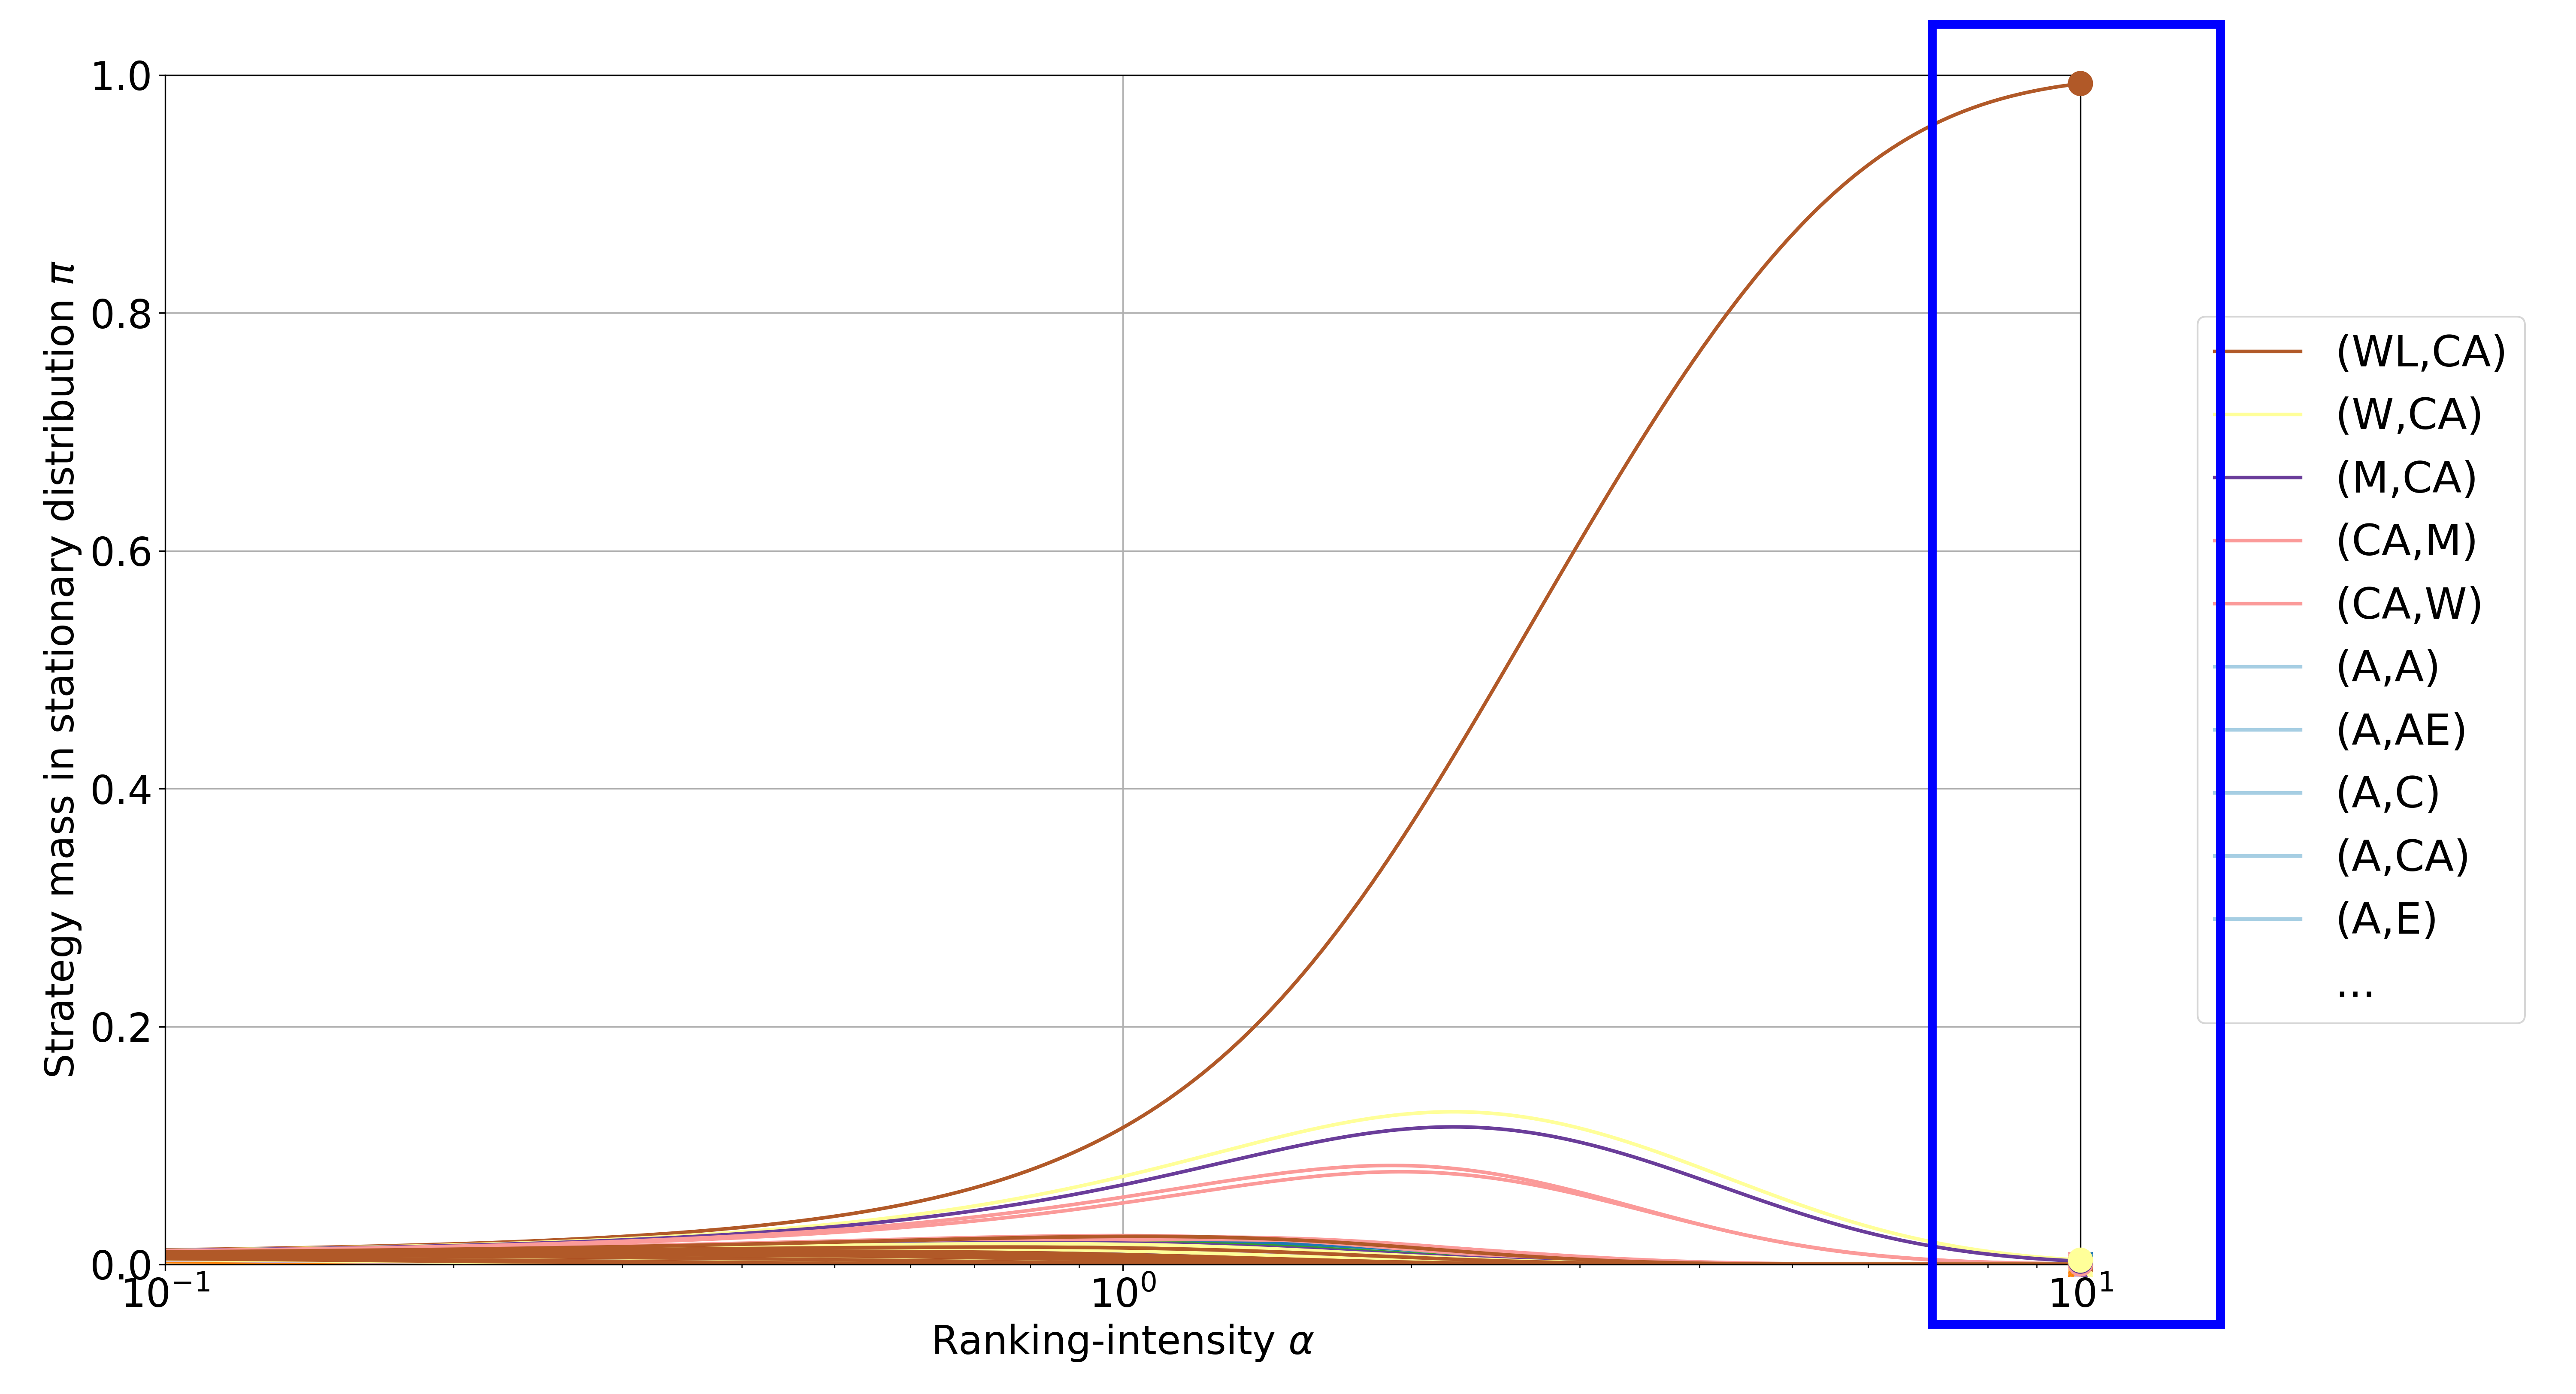
\includegraphics[width=\linewidth]{images/alpha_x_pi_10.png}
                \caption{Mass across $\alpha \in [0.1, 10]$.}
                \label{fig:alpha_x_pi_10}
            \end{subfigure}
            \caption{Effect of ranking intensity $\alpha$ on strategy profile mass in the stationary distribution $\pi$.}
            \label{fig:alpha_x_pi}
        \end{figure}
        %

        \noindent
        We plot two such graphs to observe how the mass of strategy profiles is distributed in the MCCs across different $\alpha$ values. In the stationary distribution resulting from a bigger $\alpha$, the dominant strategy profile (WL, CA) in the MCC achieves a mass of 1, with all other profiles dropping to 0. This is clearly illustrated in the second plot (see Figure~\ref{fig:alpha_x_pi_10}). However, regarding the mass distribution for a smaller range of $\alpha$, depicted n the first plot, the game has not yet converged to the final MCC.

\newpage

\subsection{Section 6}

\newpage

%%%%%%%%%%%%%%%%%%%%%%% Uncomment for the Greek Version %%%%%%%%%%%%%%%%%%%%%%%

% \section{Συμπεράσματα}

\section{Conclusions}
\cite{exampleArticle}

\newpage

%%%%%%%%%%%%%%%%%%%%%%% Uncomment for the Greek Version %%%%%%%%%%%%%%%%%%%%%%%
% \printbibliography[title={Βιβλιογραφία}]

\printbibliography

\newpage

%%%%%%%%%%%%%%%%%%%%%%% Uncomment for the Greek Version %%%%%%%%%%%%%%%%%%%%%%%
% \renewcommand\appendixpagename{Παραρτήματα}

% \begin{appendices}
%     \section*{Παράρτημα A}
% \end{appendices}

\begin{appendices}
    \section*{Appendix A}
    Ενδεικτική Δομή Διπλωματικής. Ισχύει κυρίως για διπλωματικές «Πληροφορικού» περιεχομένου που περιγράφουν κάποια υλοποίηση συστήματος. Τα κεφάλαια 2 και 3 μπορεί να συμπτυχθούν σε ένα, ανάλογα με την περίσταση – ρωτήστε τους επιβλέποντες. Το ίδιο ισχύει και για τα κεφάλαια 5 και 6. \\~\\

    \makebox[\textwidth][c]{
        \begin{tabular}{|c|l|c|}
         \hline
         Κεφάλαια & \multicolumn{1}{|c|}{Περιεχόμενο} & \multicolumn{1}{| p{3cm} |}{\centering Μέγεθος (Σελίδες)} \\
         \hline\hline
         Εξόφυλλο & Βλ. πρότυπο  & 1 \\ 
         \hline
         Αφιέρωση & Προαιρετικό & 1 \\
         \hline
         Πρόλογος & \multicolumn{1}{| p{10cm} |}{Εξήγηση του τίτλου της διπλωματικής. Λίγα λόγια για το σύστημα και γενικά για την επιστημονική περιοχή στην οποία κινείται η εργασία. Που εκπονήθηκε, υπό ποιόν καθηγητή, ευχαριστίες.}  & 1/2-1 \\
         \hline
         Περιεχόμενα & \multicolumn{1}{| p{10cm} |}{Περιεχόμενα (μέχρι και επιπέδου 3)} & 3-4 \\
         \hline
         1 Εισαγωγή & \multicolumn{1}{| p{10cm} |}{Επανάληψη προλόγου με πιο αναλυτικά λόγια Ανάλυση (1 παράγραφος) για το κάθε κεφάλαιο της εργασίας} & 2-5 \\
         \hline
         2 & \multicolumn{1}{| p{10cm} |}{Σύντομη περιγραφή του γενικότερου επιστημονικού/τεχνικού πεδίου που πραγματεύεται η διπλωματική} & 10-15 \\
         \hline
         3 & \multicolumn{1}{| p{10cm} |}{Σύντομη περιγραφή του ειδικότερου θέματος/προβλήματος που πραγματεύεται η διπλωματική} & 10-15 \\
         \hline
         4 & \multicolumn{1}{| p{10cm} |}{Σύντομη περιγραφή του εργαλείου/εργαλείων που χρησιμοποιεί η διπλωματική (αν υπάρχουν)} & 10-15 \\
         \hline
         5 & \multicolumn{1}{| p{10cm} |}{Γενικότερη (αφηρημένη) περιγραφή της λύσης που δόθηκε στο πρόβλημα (π.χ. αρχιτεκτονική του συστήματος)} & 5-10 \\
         \hline
         6 & \multicolumn{1}{| p{10cm} |}{Περιγραφή της υλοποίησης - εικόνες (screenshots), σύντομα τμήματα κώδικα (επεξηγημένα)} & 15-20 \\
         \hline
         7 & \multicolumn{1}{| p{10cm} |}{Επίλογος - Συμπεράσματα - Μελλοντική εργασία Κριτική αναφορά στα πεπραχθέντα της εργασίας Προβλήματα, Δυσκολίες που αντιμετωπίστηκαν Θέματα που δεν λύθηκαν και τίθενται ως μελλοντικός στόχος άλλων διπλωματικών} & 2-5 \\
         \hline
         Βιβλιογραφία & \multicolumn{1}{| p{10cm} |}{Βιβλία - εργασίες - Web links που χρησιμοποιήθηκαν ή κρίνονται απαραίτητα για τον αναγνώστη} & 1-2 \\
         \hline
         Παραρτήματα & \multicolumn{1}{| p{10cm} |}{Κώδικας (ολόκληρος ή σημαντικά μόνο τμήματα αν είναι μεγάλος) User Manual (αν είναι μεγάλο και δεν έχει ενσωματωθεί στο κεφάλαιο της υλοποίησης)} & 30-40 max  \\
         \hline
         \multicolumn{2}{|r|}{\textbf{ΣΥΝΟΛΟ}} & \textbf{90-130} \\
         \hline
        \end{tabular}}
\end{appendices}

\end{document}